\chapter{Using Convolutional Neural Networks for $\nu_{\mu}$ CC event classification}\label{ch:cnn_results}
\section{Classification using CNN10000}

%-----------------------------Commenting out selection I original work------------------------------------------------------------------
\begin{comment}
\subsection{Classification of MC data using Selection I Original CC-Inclusive Filter}\label{sel1orig}

\begin{figure}[htp!]
\centering
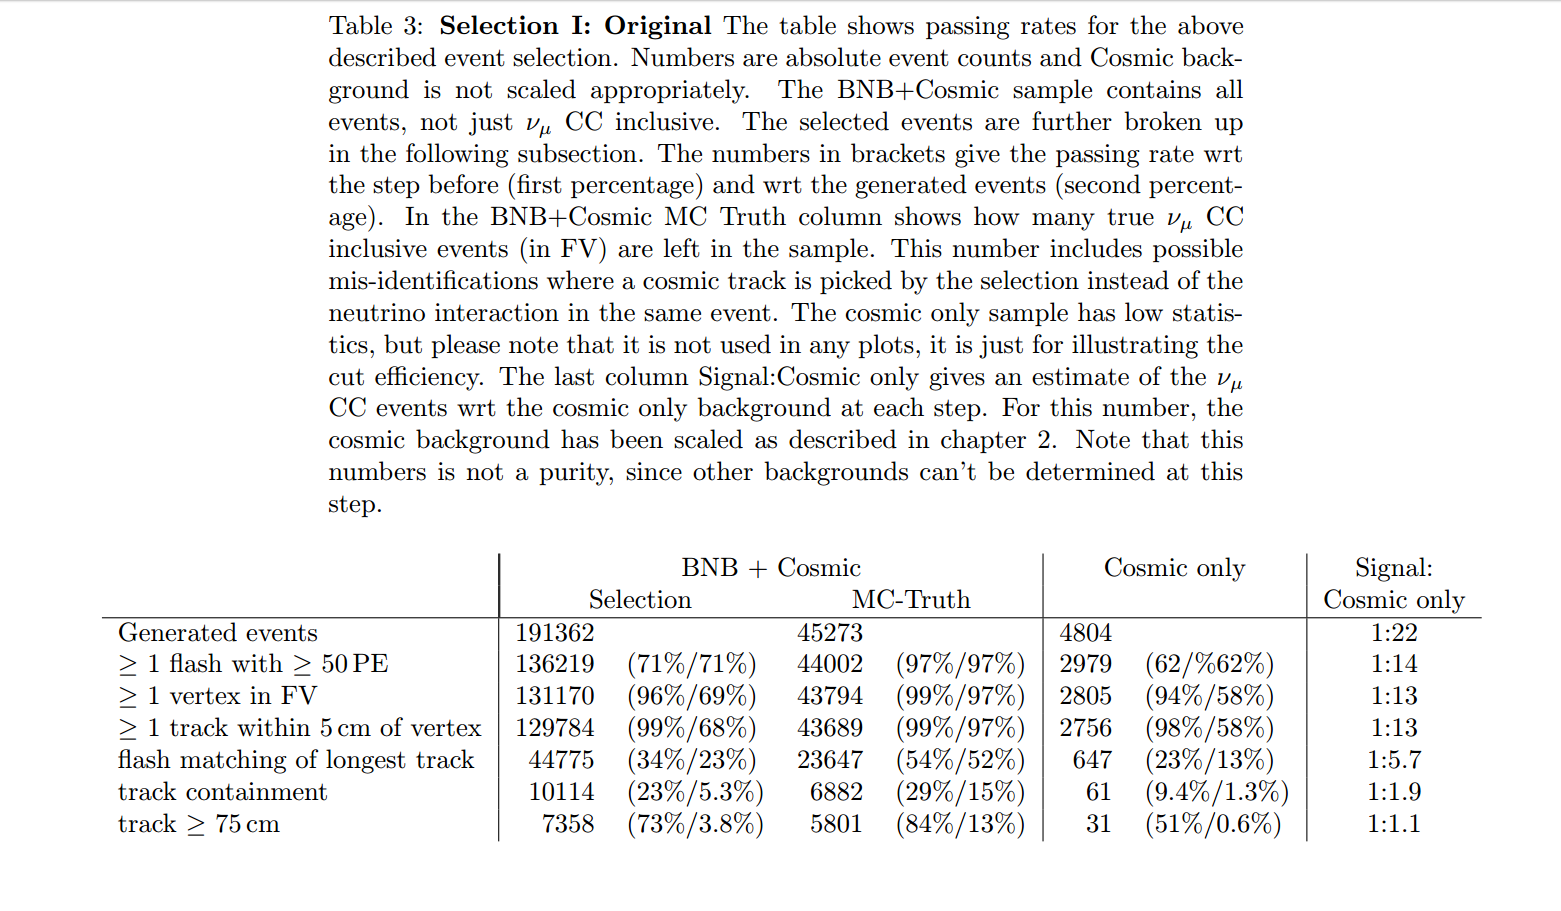
\includegraphics[width=.9\textwidth]{figs/sel1_cuts.png}
\caption{Snapshot of passing rates of Selection I from CC-Inclusive Filter} 
\label{fig:cuttable}
\end{figure}

\begin{figure}[htp!]
\centering
	\begin{subfigure}[b]{.45\textwidth}
	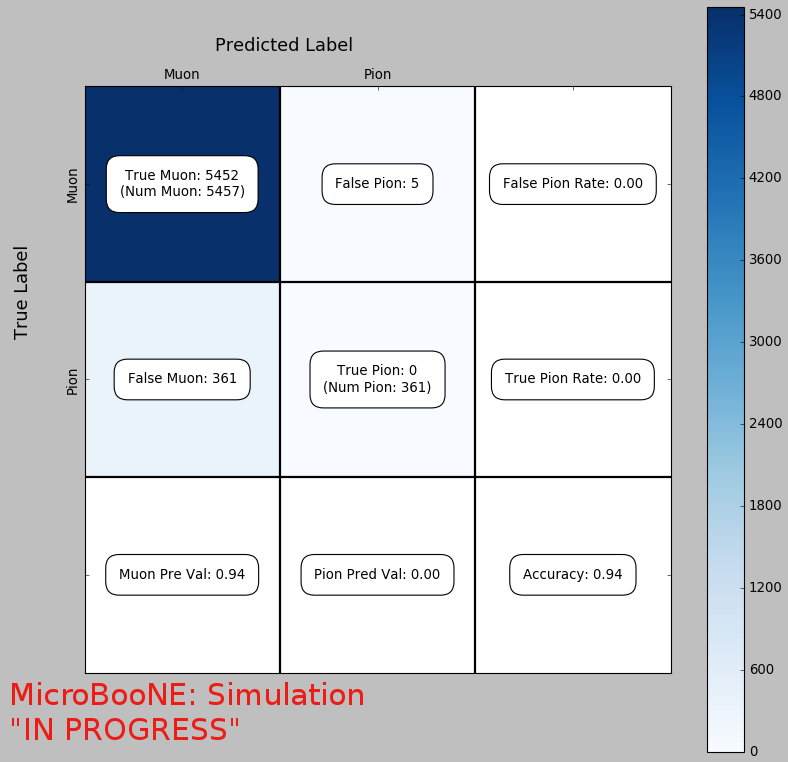
\includegraphics[width=3in,height=3in]{figs/confusion_0621_wrongnorm.png}
	\caption{Confusion Matrix showing Accuracy of CNN using data with wrong normilazion}
	\label{fig:confusion_wrongnorm}
	\end{subfigure}
	\quad
	\begin{subfigure}[b]{.45\textwidth}
	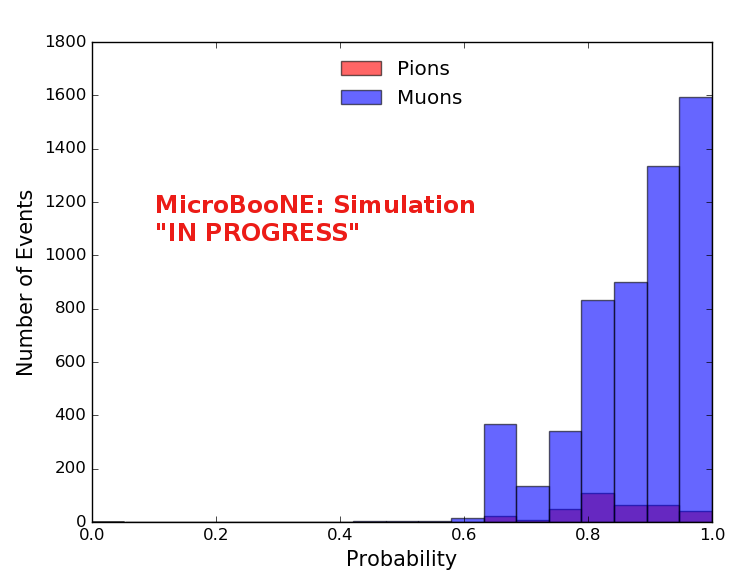
\includegraphics[width=3in,height=3in]{figs/prob_0706_wrongnorm_sel1.png}
	\caption{Probability plot showing $\mu/\pi$ separation of CNN using wrong normalization}
	\label{fig:prob_wrongnorm}
	\end{subfigure}
	\quad
	\begin{subfigure}[b]{.45\textwidth}
	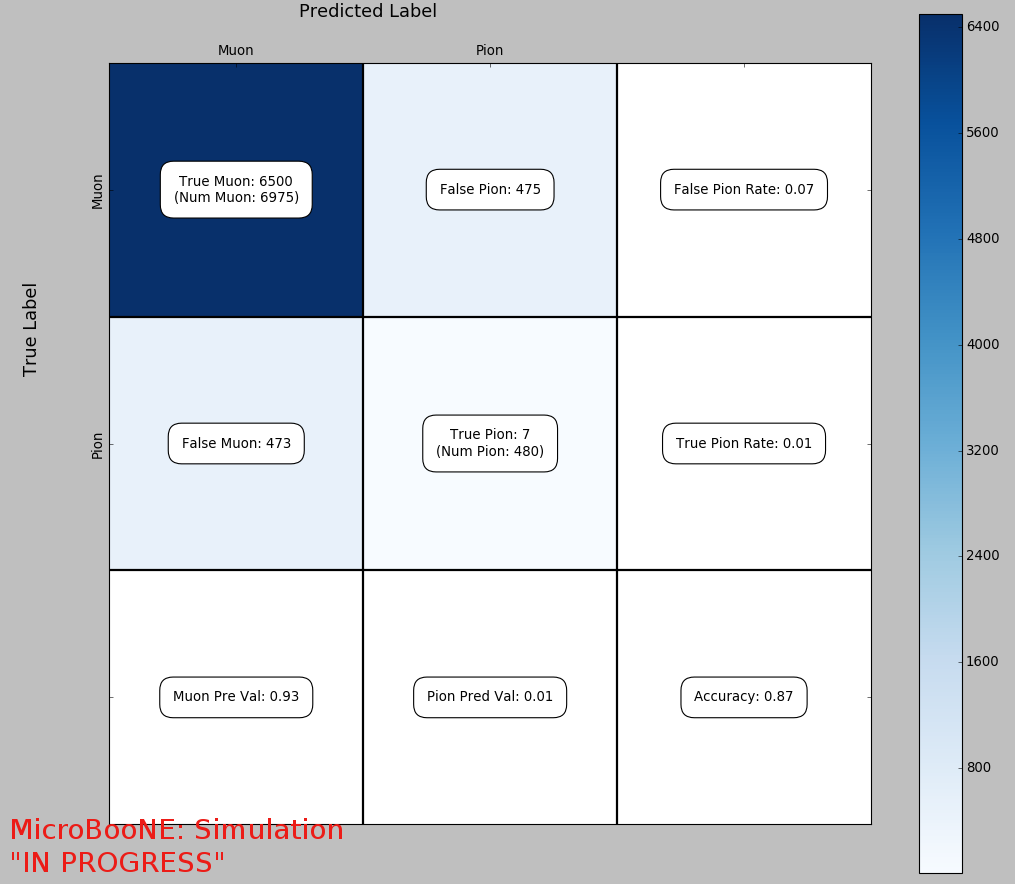
\includegraphics[width=3in,height=3in]{figs/confusion_rightnorm_0621.png}
	\caption{Confusion Matrix showing Accuracy of CNN using data with correct normilazion}
	\label{fig:confusion_rightnorm}
	\end{subfigure}
	\quad
	\begin{subfigure}[b]{.45\textwidth}
	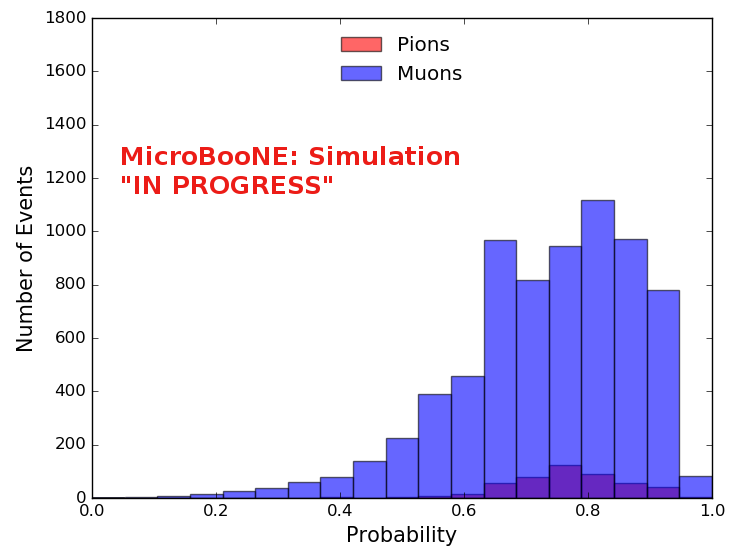
\includegraphics[width=3in,height=3in]{figs/prob_0706_rightnorm_sel1.png}
	\caption{Probability plot showing $\mu/\pi$ separation of CNN using correct normalization}
	\label{fig:prob_rightnorm}
	\end{subfigure}
	\quad
\caption{Results of CNN10000 classification of track candidate images output from cc-inclusive filter.}
\label{fig:CNN_ccnc}
\end{figure}

\begin{figure}[htp!]
\centering
	\begin{subfigure}[b]{.45\textwidth}
	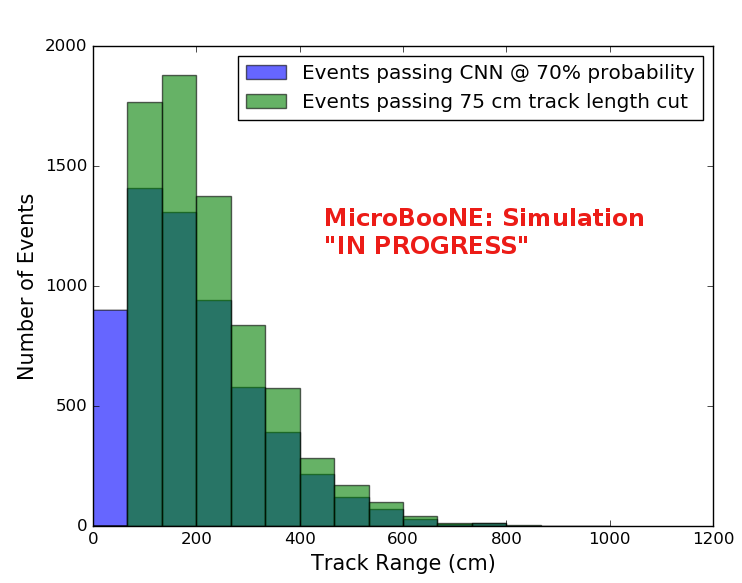
\includegraphics[width=3in,height=3in]{figs/sel1_trackrange_wrongnorm_acc70_0706.png}
	\caption{Track range distribution of events from Selection I Original passing CNN with 70\% accuracy using image data with wrong normilazion}
	\label{fig:track_wrongnorm}
	\end{subfigure}
	\quad
	\begin{subfigure}[b]{.45\textwidth}
	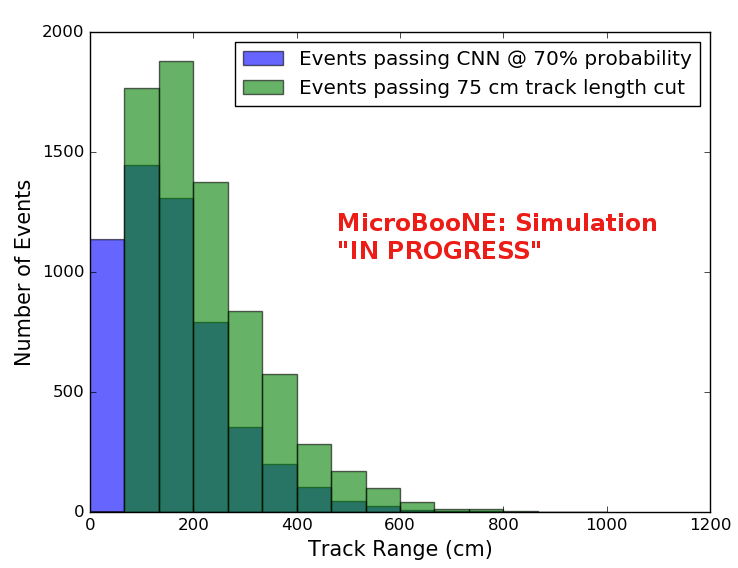
\includegraphics[width=3in,height=3in]{figs/sel1_trackrange_rightnorm_acc70_0706.png}
	\caption{Track range distribution of events from Selection I Original passing CNN with 70\% accuracy using image data with correct normilazion}
	\label{fig:track_rightnorm}
	\end{subfigure}
	\quad
	\begin{subfigure}[b]{.45\textwidth}
	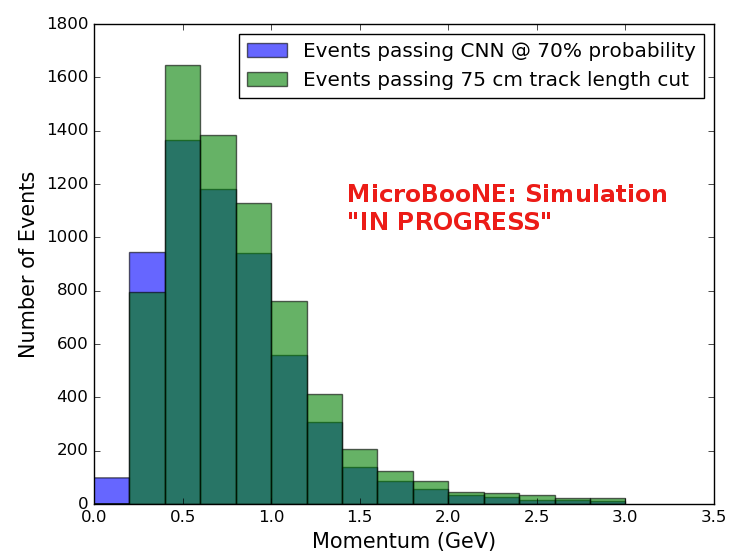
\includegraphics[width=3in,height=3in]{figs/sel1_parP_wrongnorm_acc70_0706.png}
	\caption{Momentum distribution of events from Selection I Original passing CNN with 70\% accuracy using image data with wrong normilazion}
	\label{fig:momentum_wrongnorm}
	\end{subfigure}
	\quad
	\begin{subfigure}[b]{.45\textwidth}
	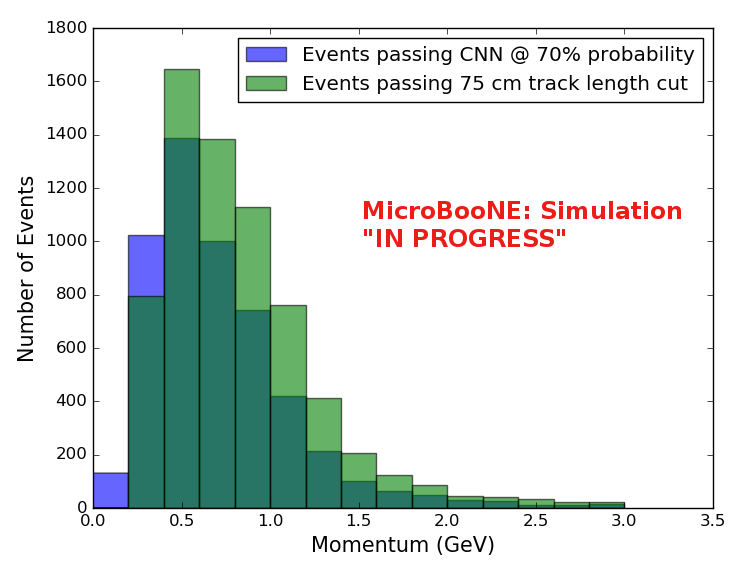
\includegraphics[width=3in,height=3in]{figs/sel1_parP_rightnorm_acc70_0706.png}
	\caption{Momentum distribution of events from Selection I Original passing CNN with 70\% accuracy using image data with correct normilazion}
	\label{fig:momentum_rightnorm}
	\end{subfigure}
	\quad
\caption{CNN10000 distributions of track candidate images output from Selection I Original cc-inclusive filter with different image data normalizations}
\label{fig:CNN_dist}
\end{figure}

The next step that was taken was to use CNN10000 to classify track candidate images that were identified by the Selection I original cc-inclusive filter described in \cite{cc-inclusive}. Passing rates for each cut in cc-inclusive filter are show in figure \ref{fig:cuttable}. For the incorrect image making normalization dataset, out of 188,880 events, 7438 passed the cut right before 75 cm track length cut which is 3.9\% of total data. Discrepancies in passing rates are due to grid submission issues, however, this dataset is used to check if changes in image making normalization affects $\mu/\pi$ separation probability due to CNN10000 being trained with incorrectly image making normalized data. For the second dataset with correct image making normalization, out of 188,880 events, 9552 events passed the cut right before the 75 cm track length cut which is 5.1\% passing rate and is comparable to figure \ref{fig:cuttable}. Intime cosmics were also run over for efficiency and purity calculations. Out of 14395 in time cosmic events, 175 passed the cut right before the 75 cm track length cut which is a passing rate of 1.2\% compared to 1.3\% shown in table \ref{table:mc} in section \ref{section:eventselection} . 

Figures \ref{fig:confusion_wrongnorm}, \ref{fig:prob_wrongnorm}, \ref{fig:confusion_rightnorm} and \ref{fig:prob_rightnorm} show the accuracy and $\mu/\pi$ separation of both the correct and incorrect normalized images. The confusion matrices are only composed of $\mu/\pi$ data. Other particles passed the cc-inclusive filter before the 75 cm track length cut and were all mis-id'ed as muons. Since CNN10000 has not seen any particles other than muons and pions, it makes sense that those get mis-id'ed. Figures \ref{fig:prob_wrongnorm} and \ref{fig:prob_rightnorm} don't have $\mu/\pi$separation comparable to \ref{fig:prob_plot}, but \ref{fig:prob_wrongnorm} does skew to higher probabilities compared to \ref{fig:prob_rightnorm}. This is to be expected and further work on quantifying the performance of CNN10000 should use the incorrect image making normalization. It is also expected that the separation isn't as defined as the testing dataset for CNN10000. CNN10000 was trained and tested using single particle muons and pions and the track candidate dataset come from BNB+Cosmic events, not to mentions all track candidates have passed the cc-inclusive filter that tags "muon-like" tracks therefore the pions in this sample look much closer in muon topology than the network has seen. Also, these images were made from wire and time ticks associated to hits from the track candidate that passed the cc-inclusive filter. This is different from the training images where a bounding box was drawn over the total $\mu$ or $\pi$ interaction. Spurious energy deposition from a $\pi-Ar$ interaction is most likely not included in the BNB+Cosmic images due to the tracking algorithm. To remedy this, the CNN needs to see more "muon-like" pions and muons and pions from a neutrino interaction passing the cc-inclusive filter as well as a larger particle variety including protons, photons and electrons. Although $\mu/\pi$ separation is lacking, CNN10000 does an excellent job of classifying muons and using higher CNN probability can increase purity. Figures \ref{fig:track_wrongnorm}, \ref{fig:track_rightnorm}, \ref{fig:momentum_wrongnorm} and \ref{fig:momentum_rightnorm} show the track and momentum distributions for these two datasets. In both sets you have an increase in data in the bin below 75 cm and at bins below 0.5 GeV. These distributions were made with events classified with 70\% probability of being a muon regardless of true particle type. 
\end{comment}
%-----------------------------Commenting out selection I original work------------------------------------------------------------------

\subsection{Classification of MC data using Selection I CC-Inclusive Filter}

After training CNN10000, it was then used to classify track candidate images that were identified by the Selection I cc-inclusive filter right before the 75 cm track length cut described in chapter \ref{ch:meas}. Passing rates for each cut in this filter are shown in table \ref{table:mc}. Out of 188,880 events, 19,112 passed the cut right before the 75 cm track length cut which is a 10.1\% passing rate and comparable to the 10\% passing rate shown in table \ref{table:mc}. Intime cosmics were also run over, out of 14,606 in time cosmics events, 302 passed the cut right before the 75 cm track length cut which is a 2.1\% passing rate comparable to the 2.7\% passing rate in the cc-inclusive tech-note. Figures \ref{fig:confusion_sel1mod} and \ref{fig:prob_sel1mod} show the accuracy and $\mu/\pi$ separation. Both plots are only composed of muons and pions due to the focus on $\mu/\pi$ separation and the fact that CNN10000 was only trained on muons and pions, however, for reference, all other particles that did pass Selection I were mis-id'ed as muons. Muons are being identified at a very high rate, while pions are all being mis-id'ed as muons. This is due in part because the pion track candidate that does pass the cc-inclusive filter right before the 75 cm track length cut has already been identified as a muon candidate, hence, at a higher muon probability. Another reason for the pion mis'id can be attributed to the training/classifying dataset difference. For training, the pion images include the whole pion interaction in argon, including any decays or nucleon scattering. The image created from a BNB+Cosmic event used for classification only includes the track candidate that passed the cc-inclusive filter right before the 75 cm track length cut.
Figure \ref{fig:sel1mod_track} shows the track range distributions of all events from Selection I being classified by the CNN as a muon with a probability of 70\% regardless of true particle type. We get entries for the CNN curve in the lowest bin and none for the 75 cm curve. To see how many true CC events were identified by CNN10000 breaking down figure \ref{fig:sel1mod_track} by event type was necessary. Figures \ref{fig:sel1mod_stackedcnn} and \ref{fig:sel1mod_stackedoriginal} show track range distributions separated by signal and various backgrounds. Particle type was not taken into consideration in these plots so true CC event images can be any track candidate particle passing Selection I cut right before track length cut including pions and protons. 

To gain an even deeper understanding on how CNN10000 is performing, plotting these distributions with only muons and pions was done due to the fact that CNN10000 was trained with only those particles for $\mu/\pi$ separation. Figures \ref{fig:sel1mod_mupi_70stackedcnn}-\ref{fig:sel1mod_mupi_90stackedcnn} show the stacked histograms of signal and background of the track range distributions with varying CNN probabilities starting from 70\% and ending at 90\% probability. With higher probabilities we get a purer sample in the lower bin but we end up losing events as well. Momentum distributions for all signal/background events are shown in figure \ref{fig:sel1mod_parP}. At CNN10000 at 70\% we introduce more NC background, however, we also get more CC events passing as well.   

\begin{figure}[htp!]
\centering
	\begin{subfigure}[b]{.45\textwidth}
	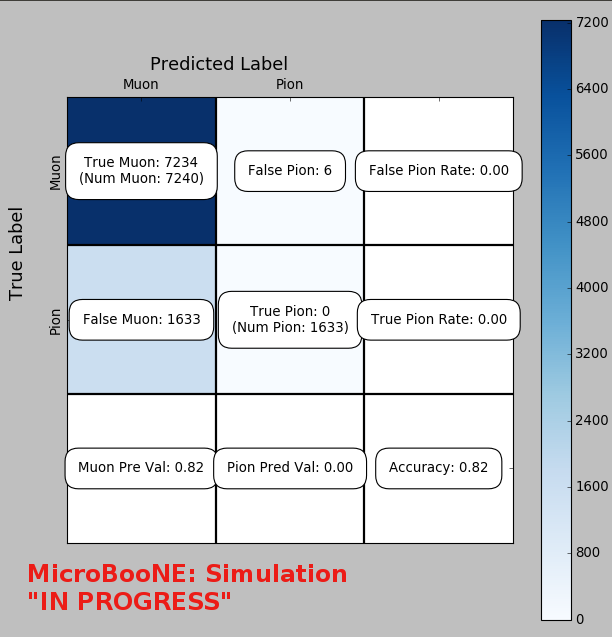
\includegraphics[width=3in,height=3in]{figs/sel1mod_confusion_wrongnorm.png}
	\caption{Confusion Matrix for CNN10000 classified events from Selection I}
	\label{fig:confusion_sel1mod}
	\end{subfigure}
	\quad
	\begin{subfigure}[b]{.45\textwidth}
	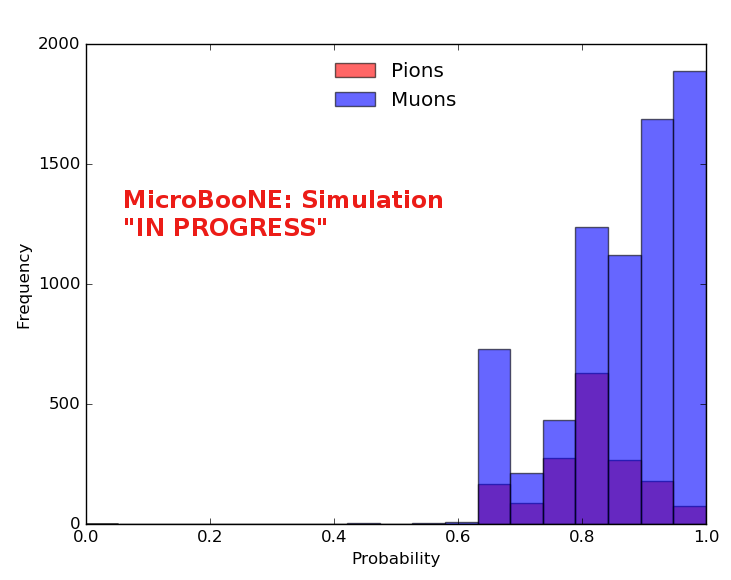
\includegraphics[width=3in,height=3in]{figs/probplot_wrongnorm_selImod.png}
	\caption{Probability plot for CNN10000 classified events from Selection I}  
	\label{fig:prob_sel1mod}
	\end{subfigure}
	\quad
\caption{Confusion matrix and probability plot of events passing Selection I cc-inclusive cuts right before 75cm track length cut}
\label{probplots}
\end{figure}

\begin{figure}[htp!]
\centering
	\begin{subfigure}[b]{.9\textwidth}
	\centering
	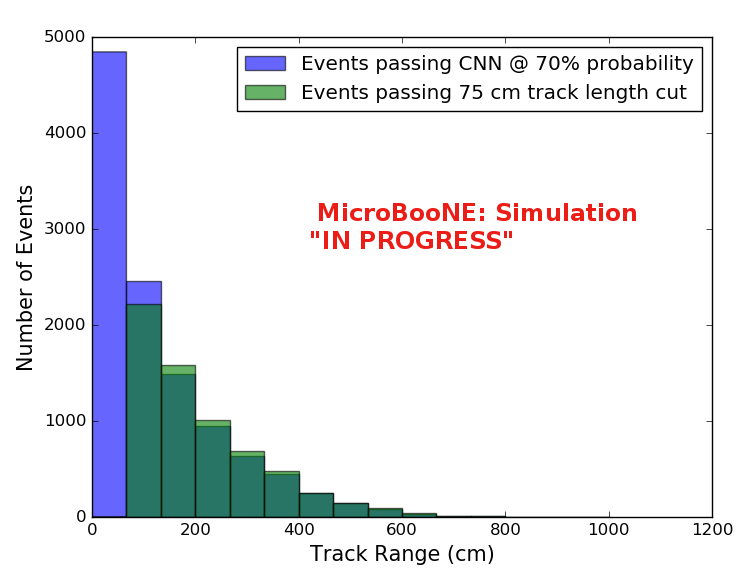
\includegraphics[width=4in,height=2.5in]{figs/sel1mod_trackrange_wrongnorm_acc70_0706.png}
	\caption{Track range distribution of events from Selection I passing CNN with 70\% accuracy}
	\label{fig:sel1mod_track}
	\end{subfigure}
	\quad
	\begin{subfigure}[b]{.45\textwidth}
	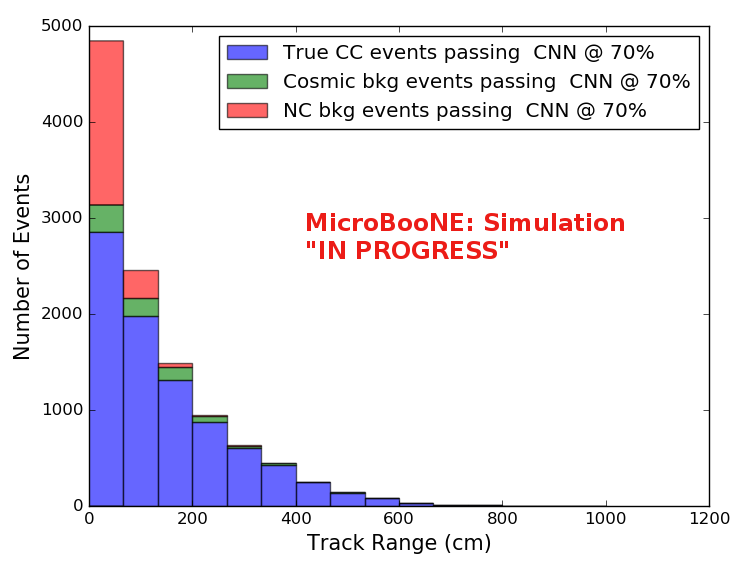
\includegraphics[width=\textwidth, height=2in]{figs/sel1mod_cnn_stackedevent_0707.png}
	\caption{Stacked signal and background track range distributions from Selection I passing CNN with 70\% accuracy}
	\label{fig:sel1mod_stackedcnn}
	\end{subfigure}
	\quad
	\begin{subfigure}[b]{.45\textwidth}
	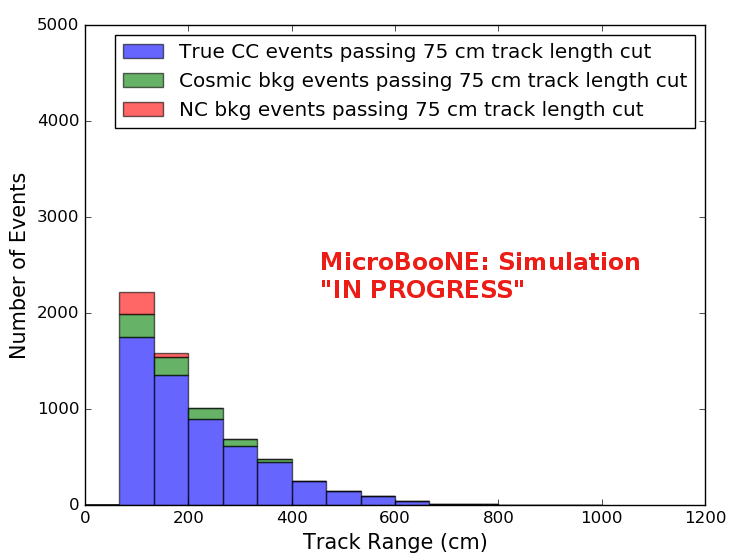
\includegraphics[width=\textwidth, height=2in]{figs/sel1mod_original_stackedevents_0707.png}
	\caption{Stacked signal and background track range distributions from Selection I passing 75 cm track length cut}
	\label{fig:sel1mod_stackedoriginal}
	\end{subfigure}
	\quad
	\begin{subfigure}[b]{.45\textwidth}
	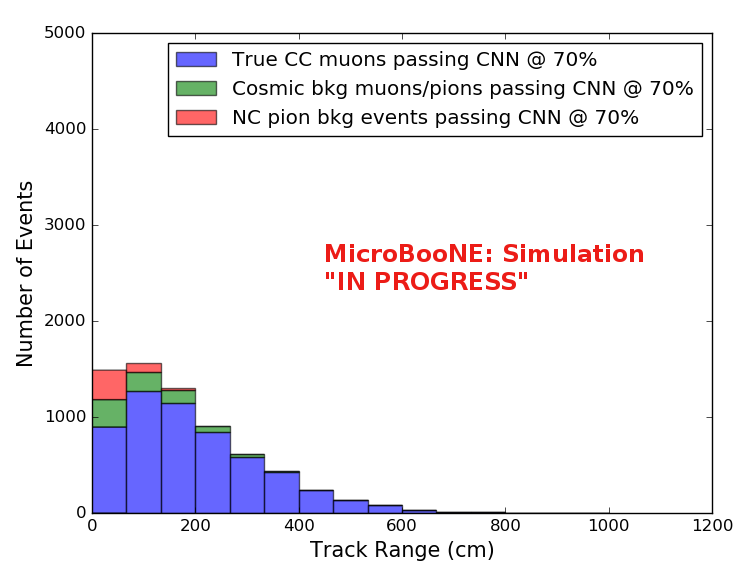
\includegraphics[width=\textwidth, height=2in]{figs/sel1mod_cnn_trackrange_mupi_acc70_0707.png}
	\caption{Stacked signal muons and background muons/pions of track range distributions from Selection I passing CNN with 70\% accuracy}
	\label{fig:sel1mod_mupi_70stackedcnn}
	\end{subfigure}
	\quad
	\begin{subfigure}[b]{.45\textwidth}
	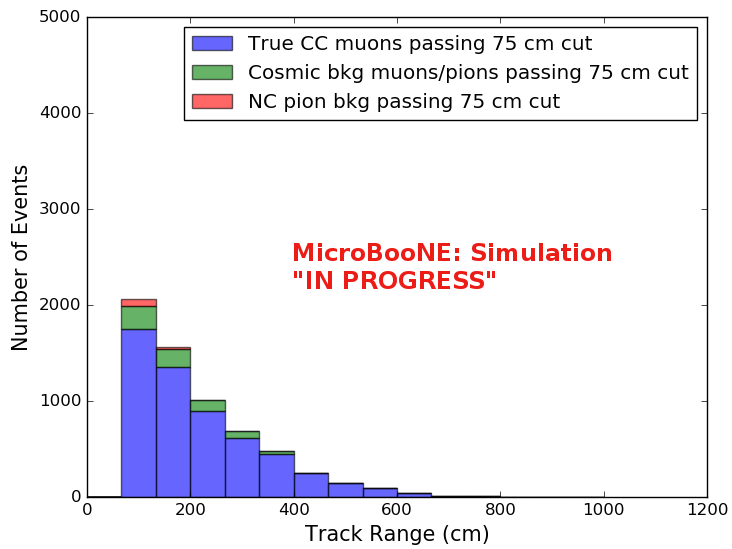
\includegraphics[width=\textwidth, height=2in]{figs/sel1mod_original_trackrange_mupi_acc70_0707.png}
	\caption{Stacked signal muons and background muons/pions of track range distributions from Selection I passing 75 cm track length cut}
	\label{fig:sel1mod_mupi_70stackedoriginal}
	\end{subfigure}
	\quad
\caption{CNN10000 distributions of track candidate images output from Selection I cc-inclusive filter}
\label{fig:sel1mod_CNN_dist}
\end{figure}



\begin{figure}[htp!]
\centering
	\begin{subfigure}[b]{.45\textwidth}
	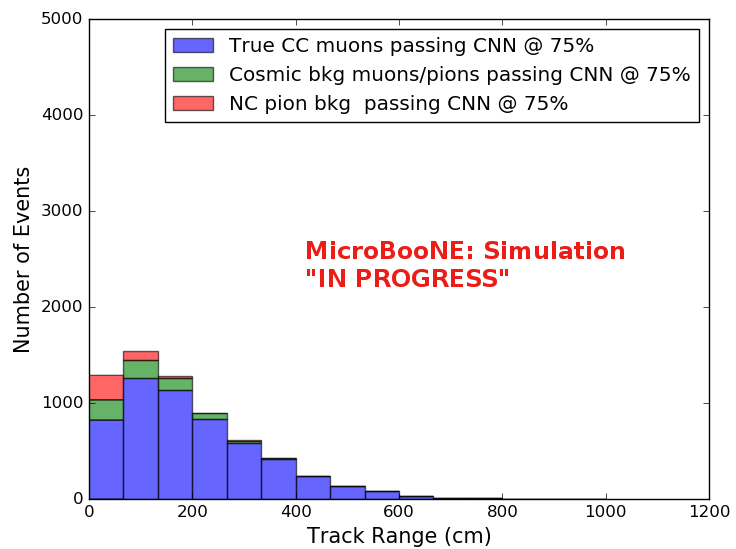
\includegraphics[width=\textwidth, height=2.5in]{figs/sel1mod_cnn_trackrange_acc75_0707.png}
	\caption{Stacked signal muons and background muons/pions of track range distributions from Selection I passing CNN with 75\% accuracy}
	\label{fig:sel1mod_mupi_75stackedcnn}
	\end{subfigure}
	\quad
	\begin{subfigure}[b]{.45\textwidth}
	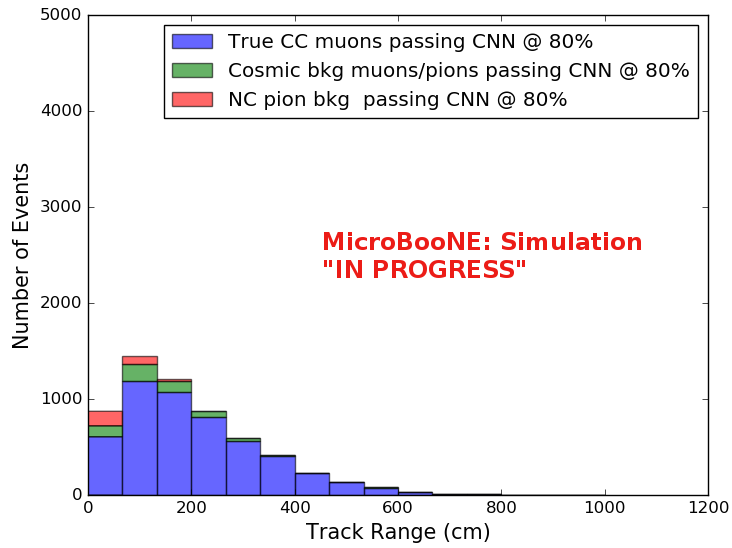
\includegraphics[width=\textwidth, height=2.5in]{figs/sel1mod_cnn_trackrange_acc80_0707.png}
	\caption{Stacked signal muons and background muons/pions of track range distributions from Selection I passing CNN with 80\% accuracy}
	\label{fig:sel1mod_mupi_80stackedcnn}
	\end{subfigure}
	\quad
	\begin{subfigure}[b]{.45\textwidth}
	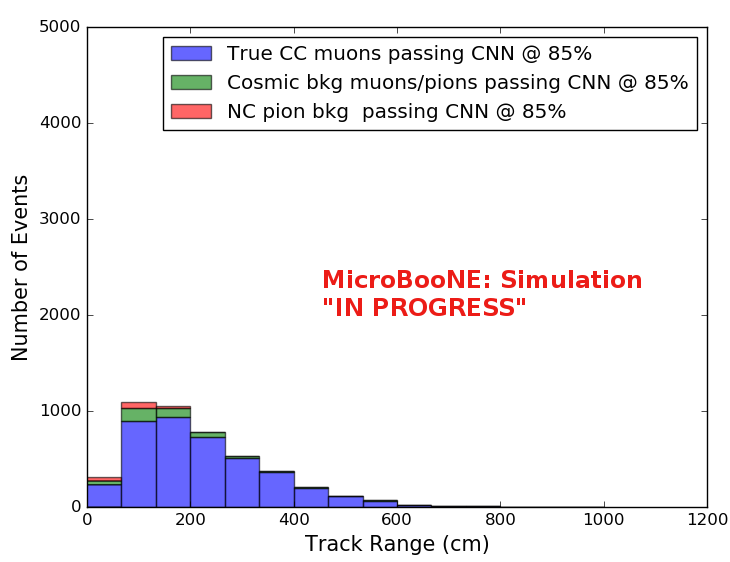
\includegraphics[width=\textwidth, height=2.5in]{figs/sel1mod_cnn_trackrange_acc85_0707.png}
	\caption{Stacked signal muons and background muons/pions of track range distributions from Selection I passing CNN with 85\% accuracy}
	\label{fig:sel1mod_mupi_85stackedcnn}
	\end{subfigure}
	\quad
	\begin{subfigure}[b]{.45\textwidth}
	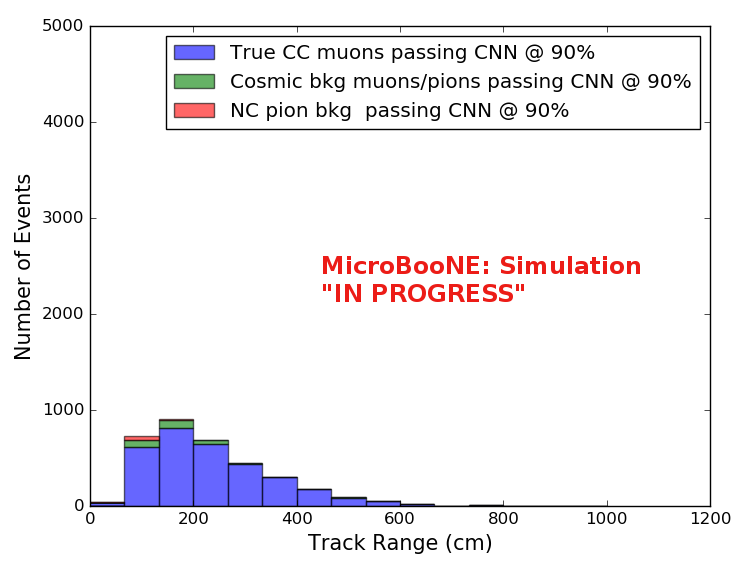
\includegraphics[width=\textwidth, height=2.5in]{figs/sel1mod_cnn_trackrange_acc90_0707.png}
	\caption{Stacked signal muons and background muons/pions of track range distributions from Selection I passing CNN with 90\% accuracy}
	\label{fig:sel1mod_mupi_90stackedcnn}
	\end{subfigure}
	\quad
\caption{CNN10000 stacked signal/background track range distributions of track candidate images output from Selection I cc-inclusive filter}
\label{fig:sel1modCNNdistacc}
\end{figure}


\begin{figure}[htp!]
\centering
	\begin{subfigure}[t]{.9\textwidth}
	\centering
	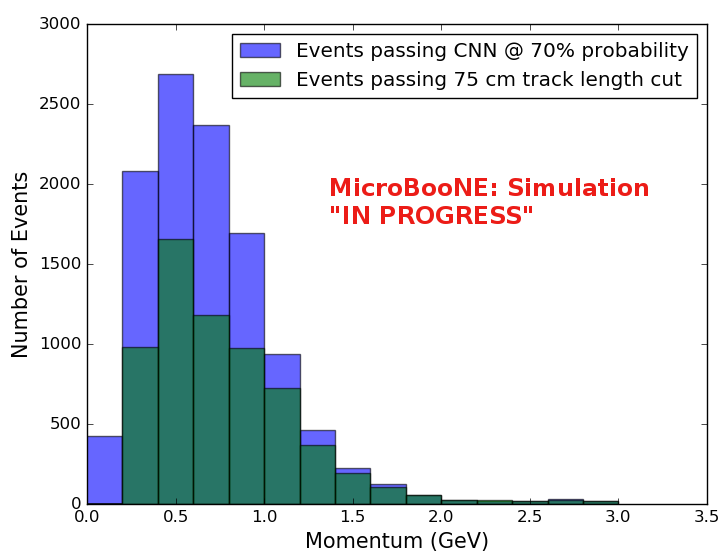
\includegraphics[width=\textwidth,height=3.5in]{figs/sel1mod_parP_wrongnorm_acc70_0706.png}
	\caption{Momentum distribution of events from Selection I passing CNN with 70\% accuracy}
	\label{fig:sel1mod_momentum}
	\end{subfigure}
	\quad
	\begin{subfigure}[t]{.45\textwidth}
	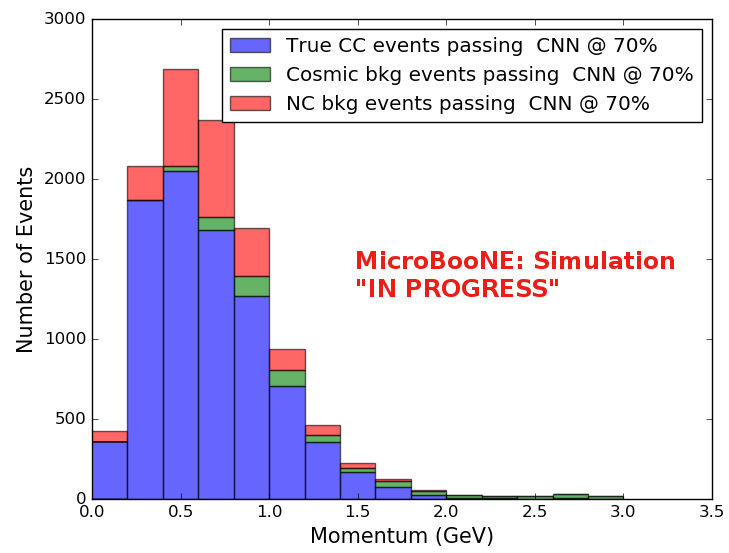
\includegraphics[width=\textwidth,height=2.5in]{figs/sel1mod_cnn_parP_stackedevents_0707.png}
	\caption{Stacked signal and background momentum distributions from Selection I passing CNN with 70\% accuracy}
	\label{fig:sel1mod_momentum_stackedcnn}
	\end{subfigure}
	\quad
	\begin{subfigure}[t]{.45\textwidth}
	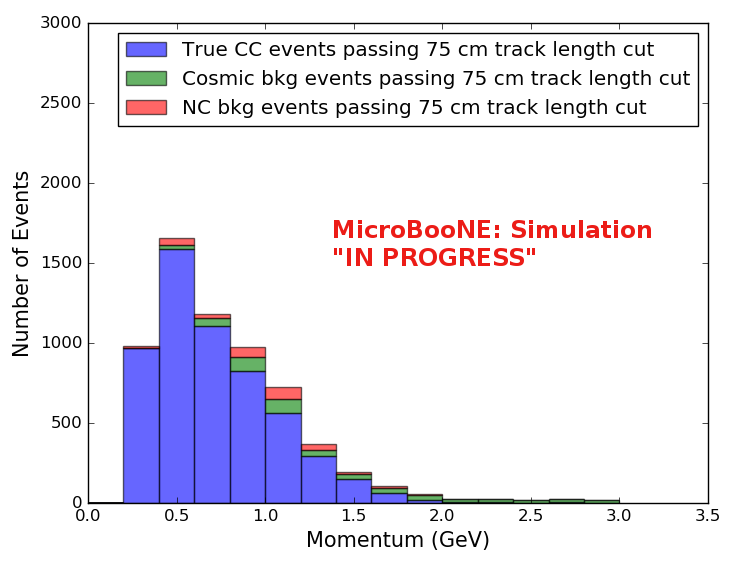
\includegraphics[width=\textwidth,height=2.5in]{figs/sel1mod_original_parP_stackedevents_0707.png}
	\caption{Stacked signal and background momentum distributions from Selection I passing 75 cm track length cut}
	\label{fig:sel1mod_momentum_stackedoriginal}
	\end{subfigure}
	\quad
\caption{CNN10000 momentum distributions of track candidate images output from Selection I cc-inclusive filter}
\label{fig:sel1mod_parP}
\end{figure}

Another check was to see if any true CC pions were passing through the cut right before the 75 cm track length cut. Figure \ref{fig:mupi} shows the comparison of the stacked track range distribution with only true CC muon signal versus the stacked distribution with true CC muons and pions signal. As you can see, we gain more events when plotting CC events with a particle type of either muons or pions due to the CNN classifying all pions in this dataset as muons. This is an interesting scenario and a sample of topologies of these images are represented in figure \ref{fig:evd}, at least 3 tracks are coming out of the vertex for these types of events. With the 75 cm track length cut, the selection is cutting event topologies like this where the pion is the tagged track candidate. Figure \ref{fig:longer_muon_badreco} has a defined longer muon track, but because of dead wires through the track, the reconstructed range is 1. less than 75 cm and 2. shorter than the reconstructed pion whose length is also less than 75 cm. This is a very interesting event, but because of issues with the tracking algorithm, the 75 cm cut would get rid of this event. The CNN was able to recover this event only because it has classified all pions as muons. Figure \ref{fig:longer_pion} shows the second case to think about, the pion, while still less than 75 cm has a reconstructed track length longer than the muon. Again, the CNN recovered this event due to pions being classified as muons. Lastly, figure \ref{fig:verylongpion} shows a pion with a reconstructed track length greater than 75 cm and the muon. These three cases show that a broader question must be asked when training the network other than is it a muon or pion. There are different routes to recover interesting events like these. One route is to ask the network ``Is it a CC event or is it an NC event?'' and obtain an image dataset consisting of whole CC/NC events that will train the network to answer this question. The other route is to ask the network ``Is this a $\mu/\pi/p/$ from a CC event or NC event and obtain an image dataset consisting of primary particles from a CC/NC event. Both these paths will be explored in future work.     

\begin{figure}[htp!]
\centering
	\begin{subfigure}[b]{.45\textwidth}
	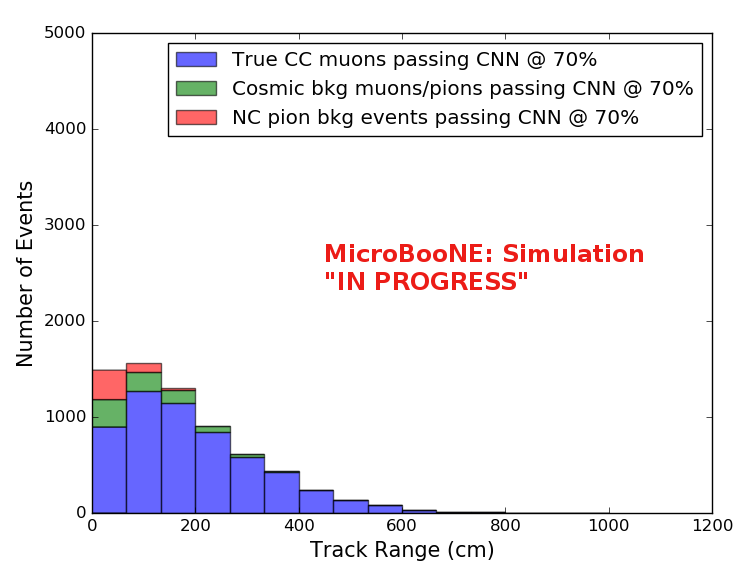
\includegraphics[width=\textwidth,height=2.5in]{figs/sel1mod_cnn_trackrange_mupi_acc70_0707.png}
	\caption{Stacked signal $\mu$/background $\mu$ and $\pi$ track range distribution of CNN @ 70\%}
	\end{subfigure}
	\quad
	\begin{subfigure}[b]{.45\textwidth}
	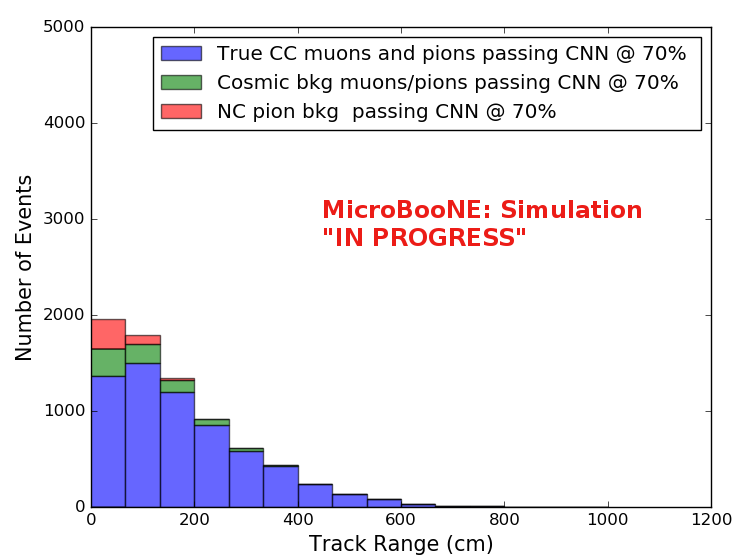
\includegraphics[width=\textwidth,height=2.5in]{figs/sel1mod_mupi_trackrange_acc70.png}
	\caption{Stacked signal $\mu \& \pi$/background $\mu \& \pi$ track range distribution of CNN @ 70\%}
	\label{fig:mupib}
	\end{subfigure}
	\quad
\caption{Track distribution comparisons of true CC muons plotted vs true CC muons and pions plotted}
\label{fig:mupi}
\end{figure}


\begin{figure}[htp!]
\centering
	\begin{subfigure}[b]{.3\textwidth}
	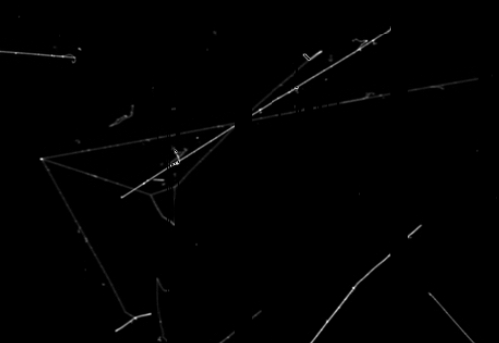
\includegraphics[width=\textwidth,height=2.5in]{figs/interesting_event.png}
	\caption{Pion reconstructed track range is less than 75 cm and longer than muon track due to dead wires}
	\label{fig:longer_muon_badreco}
	\end{subfigure}
	\quad
	\begin{subfigure}[b]{.3\textwidth}
	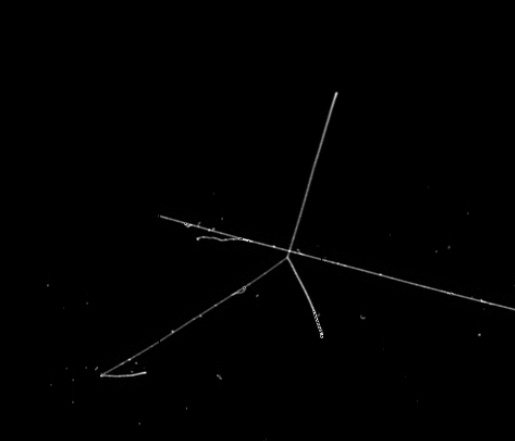
\includegraphics[width=\textwidth,height=2.5in]{figs/event2.png}
	\caption{Pion reconstructed track range is less than 75 cm and larger than muon reconstructed track}
	\label{fig:longer_pion}
	\end{subfigure}
	\quad
	\begin{subfigure}[b]{.3\textwidth}
	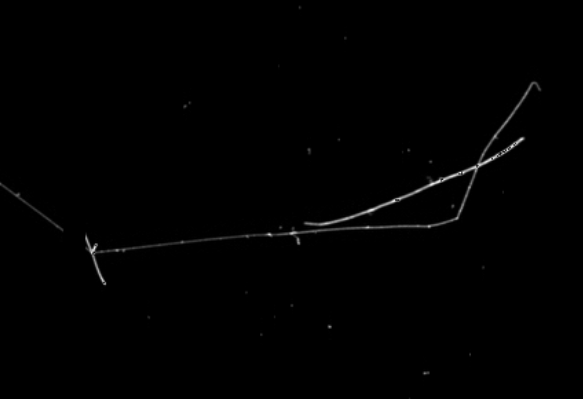
\includegraphics[width=\textwidth,height=2.5in]{figs/mupievent.png}
	\caption{Pion reconstructed track range is greater than 75 cm and larger than muon reconstructed track}
	\label{fig:verylongpion}
	\end{subfigure}
	\quad
\caption{Images of true CC events where the pion was the tagged track candidate}
\label{fig:evd}
\end{figure}

\begin{table}[htp!]
\centering
\resizebox{\textwidth}{!}{ \begin{tabular}{c||c| c c| c| c} % centered columns (4 columns)
\hline %inserts double horizontal lines
\toprule 
      && \multicolumn{2}{c}{BNB + Cosmics} & \multicolumn{1}{c}{Cosmic Only} & \multicolumn{1}{c}{Signal:}\\

      && Selection & MC Truth & &Cosmic Only \\

\midrule
75 cm Cut passing rates	& Generated Events  	       & 191362             & 45723               & 4804                & 1:22 \\ % inserting body of the table
                        & Track Containment 	       & 19391 (48\%/10\%)  & 11693 (45\%/26\%)   & 129 (38\%/2.7\%)    & 1:2.3  \\
\rowcolor{LightCyan}    & track $\geq$ 75 cm 	       & 6920 (36\%/3.6\%)  & 5780 (49\%/13\%)    & 17 (13\%/0.4\%)     & 1:0.6  \\
\hline\hline
CNN passing rates       & Generated Events  	       & 188880             & 44689               & 14606               & 1:21 \\ % inserting body of the table
		        & Track Containment 	       & 19112 ( /10\%)     & 11554 ( /26\%)      & 302 ( /2.1\%)       & 1:1.73  \\
\rowcolor{LightCyan}    & CNN cut @ 70\% Probability   & 16502 (86\%/8.7\%) & 10605 (92\%/23\%)   & 205 (68\%/14\%)     & 1:1.28  \\
\rowcolor{LightCyan}    & CNN cut @ 83\% Probability   & 7511 (46\%/4.0\%)  & 6142  (58\%/14\%)   & 32 (16\%/0.2\%)     & 1:0.4  \\
\bottomrule
\hline %inserts single line
\end{tabular}}
\caption{Comparing passing rates of CNN at different probabilities versus 75 cm track length cut: Numbers are absolute event counts and Cosmic background is not scaled appropriately. The BNB+Cosmic sample contains all events. The numbers in brackets give the passing rate wrt the step before (first percentage) and wrt the generated events (second percentage). In the BNB+Cosmic MC Truth column shows how many true $\nu_{\mu}$ CC-inclusive events (in FV) are left in the sample. This number includes possible mis-identifications where a cosmic track is picked by the selection instead of the neutrino interaction in the same event.The CNN MC True generated events were scaled wrt the MC True generated events for the 75 cm cut passing rates due to only running over 188,880 generated events versus the 191362 generated events. The last column Signal:Cosmic only gives an estimate of the $\nu_{\mu}$ CC events wrt the cosmic only background at each step. For this number, the cosmic background has been scaled as described in \cite{cc-inclusive}. Note that these numbers are not a purity, since other backgrounds can’t be determined at this step.} 
% title of Table
\label{table:passingrates} % is used to refer this table in the text
\end{table}


\begin{table}[htp!]
\centering
\resizebox{\textwidth}{!}{ \begin{tabular}{c c c|a} % centered columns (4 columns)
%\hline %inserts double horizontal lines
      &&\#Events(Fraction)  & \#Events(Fraction) \\
      &&passing Sel I & passing CNN @ 83\% Probability\\


Signal	       & $\nu_{\mu}$ CC events with true vertex in FV      & 1168(53.8\%)       & 6142(61\%)\\ % inserting body of the table
\hline\hline %inserts double horizontal lines
Backgrounds    & Cosmics Only Events                               & 725(33.4\%)       & 2582(26\%)\\ % inserting body of the table
               & Cosmics in BNB Events                             & 144(6.6\%)       & 492(4.9\%)\\ % inserting body of the table
               & NC Events                                         & 75(3.5\%)        & 778(7.7\%)\\ % inserting body of the table
               & $\nu_e$ and $\bar{\nu}_e$ Events                  & 4(0.2\%)        & 32(0.3\%)\\ % inserting body of the table
               & $\bar{\nu}_{\mu}$  Events                         & 40(1.8\%)         & 67(0.7\%)\\ % inserting body of the table
\end{tabular}}
\caption{Signal and background event numbers of Selection I and Selection I with CNN cut estimated from a BNB+Cosmic sample and Cosmic only sample normalized to $5*10^{19}$ PoT. The last column gives the fraction of this signal or background type to the total selected events per CNN probability.} 
\label{table:purity} % is used to refer this table in the text
\end{table}

Table \ref{table:passingrates} shows the passing rates for the 75 cm track length cut and the CNN cut at 70\% and 83\%. The passing rates at the track containment level for the 75 cm track length cut compared to the CNN are comparable with only a 0.6\% difference in the in time cosmic bin which may be due in part to the larger in time cosmic statistics used for the CNN dataset. These passing rates need to be comparable to then be able to compare the passing rates after the CNN cut to the 75 cm cut. Again, the same BNB+Cosmic sample was used for both Selection I with 75 cm cut and Selection I with CNN cut. As it stands, a CNN cut at 83\% probability has a MC true CC event passing rate of 14\% compared to the 13\% passing rate of the 75 cm track length cut. The Signal:Cosmic Only background is also reduced from 1:0.6 to 1:0.4 The total passing rate is also higher than the 75 cm cut, 3.6\% vs 4.0\%. Table \ref{table:purity} shows the breakdown of signal and backgrounds for the CNN at the different probabilities. We have a 61\% signal passing rate with the CNN cut @ 83\% versus the 53.8\% signal passing rate of the 75 cm cut. 

Based on these numbers, the following performance values of the selection with 75 cm cut versus selection with CNN @ 83\% probability cut were calculated:
\begin{itemize}
\item Efficiency: Number of selected true $\nu_{\mu}$ CC events divided by the number of expected true $\nu_{\mu}$ CC events with interaction in the FV.
\begin{itemize}
\item Selection I: 12.3\% 
\item Selection I with CNN10000 cut @ 83\% probability: 14\% 
\end{itemize}
\item Purity: Number of selected true $\nu_{\mu}$ CC events divided by sum of itself and the number of all backgrounds.
\begin{itemize}
\item Selection I: 53.8\% 
\item Selection I with CNN10000 cut @ 83\% probability: 61\% 
\end{itemize}
\end{itemize}

Lastly, figure \ref{fig:sel1mod_cnnperformance} shows a more representative performance of the CNN. Due to the fact that the CNN was trained on muons and pions, showing the performance of CC muon events versus NC pion events with respect to CNN probability gives a better picture of how the network is performing. Figure \ref{fig:sel1mod_cnnperformance} shows that at 83\% we are below the 75 cm cut NC pion threshold and still above the CC muon threshold. Using 83\% probability not only reduced the NC pion background, it also dramatically reduced the intime cosmics and cosmics in the BNB. Figure \ref{fig:sel1mod_83} shows the track range of signal muons and pions compared to background muons and pions from cosmic rays or NC interactions. Comparing figure \ref{fig:sel1mod_83} to \ref{fig:mupib} you can see the reduction in both the cosmic and NC backgrounds.  

\begin{figure}[htp!]
\centering
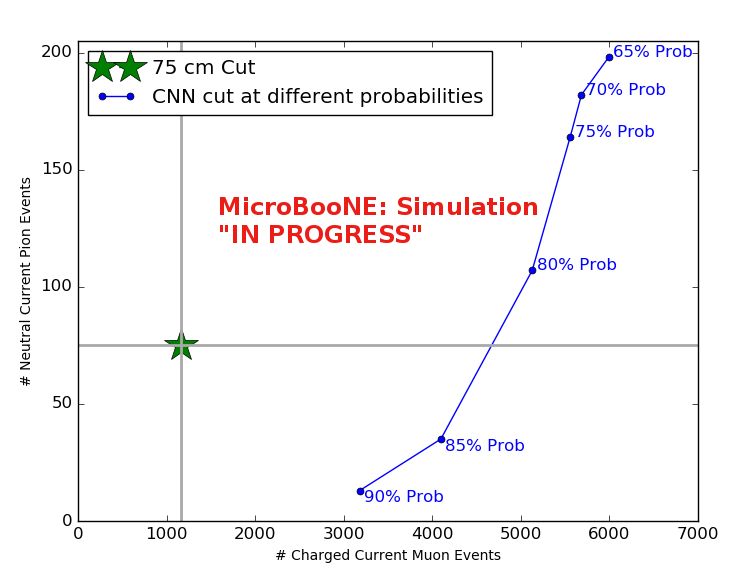
\includegraphics[width=3in,height=2.5in]{figs/cnn_performance.png}
\caption{CNN performance of classified muons and pions compared to the already implemented 75 cm track length cut}
\label{fig:sel1mod_cnnperformance}
\end{figure}

\begin{figure}[htp!]
\centering
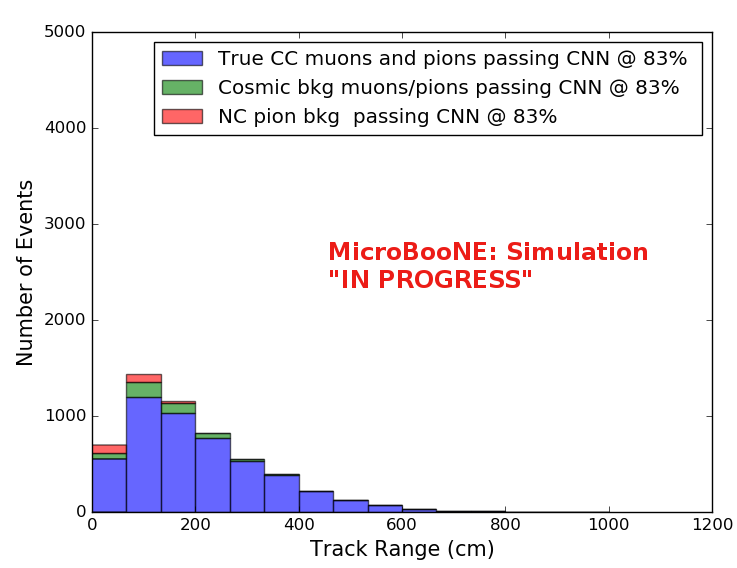
\includegraphics[width=3in,height=2.5in]{figs/sel1mod_trackrange_acc83.png}
	\caption{Stacked signal $\mu \& \pi$/background $\mu \& \pi$ track range distribution of CNN @ 83\%}
\label{fig:sel1mod_83}
\end{figure}
\subsection{Conclusions of CNN10000 classification of MC data}

It was shown that even though CNN10000 was trained with single particle generated muons and pions, it performs fairly well at classifying track candidate images from BNB+Cosmic events. Events have been regained below the 75 cm track length cut and the momentum and track range distributions have similar shapes to the distributions of Selection I. Efficiencies and purities were calculated for Selection I events before 75 cm track length cut  with the CNN at 83\% probability and are 14\% and 62\% respectively. Although the CNN doesn't have separation between muons and pions and although all particles passing CNN are classified as muon, increasing CNN probability allows us to increase the purity as well as maintain an efficiency comparable to the 75 cm track length cut all while recovering events below that 75 cm cut. Out of the 6142 events that passed the CNN @ 83\% 1470 events were below the 75 cm cut, a recovery of 3.3\% of data excluded by the 75 cm cut with a purity of 15\% which is better than Selection I. Although these numbers are low, it is an improvement from the selecion I in both total efficiency and purity and an increase in phase space by recovering these events. 

\section{Classification using CNN100000}
For classification of BNB+Cosmics and data using CNN100000, images were made from track candidates that passed the Selection I filter, however, unlike for classifying BNB+Cosmics using CNN10000, the classification of CNN100000 went further up Selection I's cut chain. For CNN100000, steps 5 through 8 seen in section \ref{section:eventselection} were removed. The image making algorithm would then create multiple images per event of pixels corresponding to each track associated to the flattest vertex candidate in the fiducial volume. One of the findings of CNN10000 was the possibility of recovering interesting events in which a pion from a cc-inclusive event is tagged as the track candidate of interest. This was the reason for trying to expand on what a convolutional neural network could accomplish. By allowing the CNN to particle ID all track associated with the vertex candidate, we allow the selection to contain the interesting events that were cut out in Selection I due to the cc pion track being chosen as the track candidate. Figure \ref{fig:cnn100000_image} shows the image making algorithm for BNB+Cosmic images. The classification algorithm would then particle ID each image in an event. If at least one of the images is identified as a muon by the CNN, the event is then classified as a $\nu_{\mu}$ event. The image with the highest muon probability is then chosen to be the track candidate and used for kinematic distribution purposes. The CNN's selection and efficiency can be tuned by increasing the muon probability of the muon track candidate image. The results of using CNN100000 to classify BNB+Cosmics will be discussed in the next sections. 

\begin{figure}[htp!]
\centering
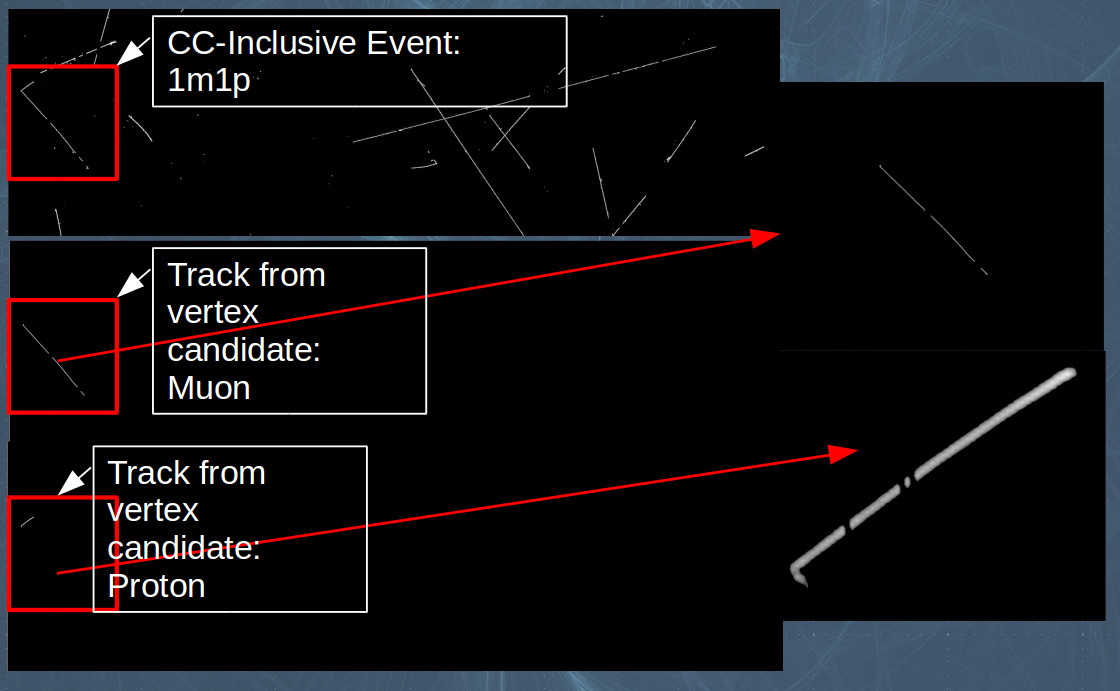
\includegraphics[width=\textwidth]{figs/cnn100000_image.png}
\caption{Image making steps used for classifying BNB+Cosmic events using CNN100000} 
\label{fig:cnn100000_image}
\end{figure}

\subsection{Classification of MC data using Selection I CC-Inclusive Filter}
After classifying all BNB+Cosmic and in time cosmic events, an efficiency vs purity curve was created for various muon probabilities to choose a probability that would increase both efficiency and purity of Selection I. This is shown in figure \ref{fig:roc}. Selection I and Selection II are also shown on this curve. At 85\% probability, both the efficiency and purity is better than both Selection I and Selection II therefore is the chosen muon probability. Although the efficiency and purity of CNN100000 have a vast increase from Selection I, making sure the truth kinematic distributions between the two selections is an important thing to check to make sure one selection isn't focusing on a different phase space than the other. Also applying CNN100000 to data to see if it responds similarly is important. 

\begin{figure}[htp!]
\centering
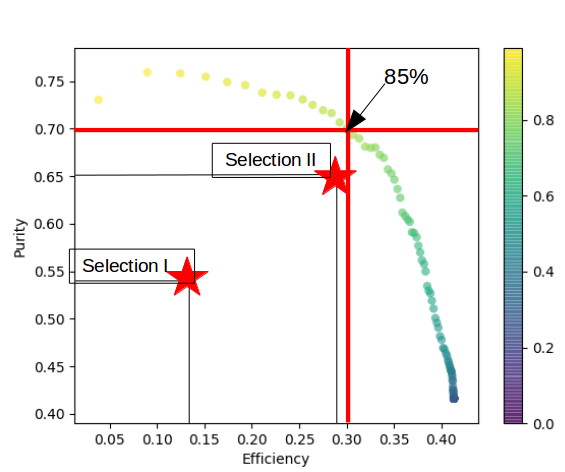
\includegraphics[width=.5\textwidth]{figs/roc_cnn_selI&II.png}
\caption{Efficiency vs Purity curve for various CNN100000 muon probabilities. At 85\% muon probability, the efficiency is 30\% and the purity is 70\%} 
\label{fig:roc}
\end{figure}

Figure \ref{fig:truthkinematics} are the true kinematic distributions for the true cc-inclusive events that passed the CNN100000 (blue) at 85\% muon probability as well as the cc-inclusive events that passed the Selection I filter (red).  

\begin{figure}[htp!]
\centering
	\begin{subfigure}[b]{.475\textwidth}
	\centering
		\includegraphics[width=\textwidth]{../bnbcosmic_output/cnn_85_trackrangedist.png}
		\caption{Track range distribution for events passing CNN10000 $\geq 85\%$ and the Selection I filter.} 
		\label{fig:cnn85trackrange}
	\end{subfigure}
	\quad
	\begin{subfigure}[b]{.475\textwidth}
	\centering
		\includegraphics[width=\textwidth]{../bnbcosmic_output/cnn_85_truecosthetadist.png}
		\caption{$Cos(\theta)$ distribution for events passing CNN100000 $\geq 85\%$ and the Selection I filter.} 
		\label{fig:cnn85costheta}
	\end{subfigure}
	\quad
	\begin{subfigure}[b]{.475\textwidth}
	\centering
		\includegraphics[width=\textwidth]{../bnbcosmic_output/cnn_85_truephidist.png}
		\caption{$\phi$ distribution for events passing CNN100000 $\geq 85\%$ and the Selection I filter.} 
		\label{fig:cnn85phi}
	\end{subfigure}
	\quad
	\begin{subfigure}[b]{.475\textwidth}
	\centering
		\includegraphics[width=\textwidth]{../bnbcosmic_output/cnn_85_momentumdist.png}
		\caption{Momentum distribution for events passing CNN100000 $\geq 85 \%$ and the Selection I filter.} 
		\label{fig:cnn85momentum}
	\end{subfigure}
\caption{Truth kinematic distributions of events passing CNN100000 and Selection I. The red corresponds to the Selection I passing events and blue to the CNN100000 passing events.}
\label{fig:truthkinematics}
\end{figure}

The shapes of the true kinematic distributions are mostly comparable for CNN100000 and Selection I, however the CNN100000 curve has more events passing at muon probability 85\% compared to the Selection I filter. This is due to the removal of the containment cut. You can also see entries for cc-inclusive events at the lowest track range bin for CNN100000 that isn't there for the Selection I filter. Although the muon probability is high, we are still able to recover events with low track candidate track range. Another thing to note in the track range plot is that the peak for CNN100000 is shifted to a higher track range compared to Selection I. This peak shift can also be seen in the momentum distribution plot. Again, a hypothesis for this shift is due to the lack of containment for the tracks, this has been explored and will be discussed. 

\begin{figure}[htp!]
\centering
	\begin{subfigure}[b]{.475\textwidth}
	\centering
		\includegraphics[width=\textwidth]{../bnbcosmic_output/cc_trackrangedist_stacked.png}
		\caption{Track range distribution for events passing Selection I filter.} 
		\label{fig:cctrackstacked}
	\end{subfigure}
	\quad
	\begin{subfigure}[b]{.475\textwidth}
	\centering
		\includegraphics[width=\textwidth]{../bnbcosmic_output/cnn_85_trackrangedist_stacked.png}
		\caption{Track range distribution for events passing CNN100000 $\geq 85\%$.} 
		\label{fig:cnn85trackstacked}
	\end{subfigure}
\caption{Truth stacked event type track range distribution of events passing Selection I (left) and CNN100000 (right). Different event types are CCQE (green), CCRES (blue), CCDIS (yellow), CCCOH (red).}
\label{fig:trackstacked}
\end{figure}

\begin{figure}[htp!]
\centering
	\begin{subfigure}[b]{.475\textwidth}
	\centering
		\includegraphics[width=\textwidth]{../bnbcosmic_output/cc_momentumdist_stacked.png}
		\caption{Momentum distribution for events passing Selection I.} 
		\label{fig:ccmomentumstacked}
	\end{subfigure}
	\quad
	\begin{subfigure}[b]{.475\textwidth}
	\centering
		\includegraphics[width=\textwidth]{../bnbcosmic_output/cnn_85_momentumdist_stacked.png}
		\caption{Momentum distribution for events passing CNN100000 $\geq 85\%$.} 
		\label{fig:cnn85momentumstacked}
	\end{subfigure}
\caption{Truth stacked event type momentum distribution of events passing Selection I (left) and CNN100000 (right). Different event types are CCQE (green), CCRES (blue), CCDIS (yellow), CCCOH (red).}
\label{fig:momentumstacked}
\end{figure}

\begin{figure}[htp!]
\centering
	\begin{subfigure}[b]{.475\textwidth}
	\centering
		\includegraphics[width=\textwidth]{../bnbcosmic_output/cc_costhetadist_stacked.png}
		\caption{$Cos(\theta)$ distribution for events passing Selection I filter.} 
		\label{fig:cccosthetastacked}
	\end{subfigure}
	\quad
	\begin{subfigure}[b]{.475\textwidth}
	\centering
		\includegraphics[width=\textwidth]{../bnbcosmic_output/cnn_85_costhetadist_stacked.png}
		\caption{$Cos(\theta)$ distribution for events passing CNN100000 $\geq 85\%$.} 
		\label{fig:cnn85costhetastacked}
	\end{subfigure}
\caption{Truth stacked event type $cos(\theta)$ distribution of events passing Selection I (left) and CNN100000 (right). Different event types are CCQE (green), CCRES (blue), CCDIS (yellow), CCCOH (red).}
\label{fig:costhetastacked}
\end{figure}

\begin{figure}[htp!]
\centering
	\begin{subfigure}[b]{.475\textwidth}
	\centering
		\includegraphics[width=\textwidth]{../bnbcosmic_output/cc_phidist_stacked.png}
		\caption{$\phi$ distribution for events passing Selection I.} 
		\label{fig:ccphistacked}
	\end{subfigure}
	\quad
	\begin{subfigure}[b]{.475\textwidth}
	\centering
		\includegraphics[width=\textwidth]{../bnbcosmic_output/cnn_85_phidist_stacked.png}
		\caption{$\phi$ distribution for events passing CNN100000 $\geq 85\%$.} 
		\label{fig:cnn85phistacked}
	\end{subfigure}
\caption{Truth stacked event type phi distribution of events passing Selection I (left) and CNN100000 (right). Different event types are CCQE (green), CCRES (blue), CCDIS (yellow), CCCOH (red).}
\label{fig:phistacked}
\end{figure}
Figures \ref{fig:trackstacked} through \ref{fig:phistacked} compare the stacked event type distributions between the Selection I filter and the CNN100000. The percentage of CCQE events that passed Selection I is 51\% compared to 62\% for CNN100000. For CCRES, Selection I had a passing rate of 37\% compared to 29\% for CNN100000. The CCDIS passing rate was 11\% and 9\% for Selection I and CNN100000 respectively. Lastly, the CCCOH rate was 1\% and 0.9\% for Selection I and CNN100000 respectively. A larger percentage of CCQE events are passing the CNN100000 compared to Selection I, an increase of 9\%. CCQE is the dominant interaction for $\nu_{\mu}$ events with neutrino energy $<1$ GeV, so being able to recover events below Selection I's 75 cm track range cut may be the reason for the increase in CCQE events. 
  
Figure \ref{fig:vertex} shows the vertex positions for the true cc-inclusive events passing the CNN100000 (blue) and the Selection I (red) filter. Again, the shape distributions are comparable among the two selections other than a higher passing rate due to the lack of track containment for CNN100000.  
\begin{figure}[htp!]
\centering
	\begin{subfigure}[b]{.55\textwidth}
	\centering
		\includegraphics[width=\textwidth]{../bnbcosmic_output/cnn_85_trackstartXdist.png}
		\caption{X Vertex Position} 
		\label{fig:cnn85vertexX}
	\end{subfigure}
	\quad
	\begin{subfigure}[b]{.55\textwidth}
	\centering
		\includegraphics[width=\textwidth]{../bnbcosmic_output/cnn_85_trackstartYdist.png}
		\caption{Y Vertex Position} 
		\label{fig:cnn85vertexY}
	\end{subfigure}
	\quad
	\begin{subfigure}[b]{.55\textwidth}
	\centering
		\includegraphics[width=\textwidth]{../bnbcosmic_output/cnn_85_trackstartZdist.png}
		\caption{Z Vertex Position} 
		\label{fig:cnn85vertexZ}
	\end{subfigure}
\caption{Vertex position for X, Y and Z of true cc-inclusive events passing CNN100000 and Selection I}
\label{fig:vertex}
\end{figure}


\subsection{Classification of MicroBooNE data using Selection I CC-Inclusive Filter}
After checking to make sure CNN100000 truth kinematic distributions looked similar to Selection I, I moved on to use CNN100000 to classify on-beam and off-beam MicroBooNE data. Figures \ref{fig:datatrackrange} through \ref{fig:dataZ} show the different kinematic distributions for on-beam and off-beam data that passed CNN100000 at 80\% muon probability. Comparing BNB+Cosmic truth distributions to MicroBooNE data distributions, the first thing to note is the peaks around $\pm\pi/2$ in the $\phi$ distribution, figure \ref{fig:dataphi} compared to a valley in figure \ref{fig:cnn85phi}. The $\pm\pi/2$ $\phi$ regions, being vertical to the beam direction, are dominated by cosmics. The $\phi$ data distribution points to an excess of cosmics passing CNN100000. 
\begin{figure}[htp!]
\centering
\includegraphics[width=.6\textwidth]{../bnbcosmic_output/data85_trackrangedist.png}
\caption{Track range distribution for on-beam (blue) and off-beam (red) data at CNN10000 $\geq 85\%$} 
\label{fig:datatrackrange}
\end{figure}

\begin{figure}[htp!]
\centering
\includegraphics[width=.6\textwidth]{../bnbcosmic_output/data85_Thetadist.png}
\caption{$Cos(\theta)$ distribution for on-beam (blue) and off-beam (red) data at CNN10000 $\geq 85\%$} 
\label{fig:datatheta}
\end{figure}

\begin{figure}[htp!]
\centering
\includegraphics[width=.6\textwidth]{../bnbcosmic_output/data85_Phidist.png}
\caption{$\phi$ distribution for on-beam (blue) and off-beam (red) data at CNN10000 $\geq 85\%$} 
\label{fig:dataphi}
\end{figure}

\begin{figure}[htp!]
\centering
\includegraphics[width=.6\textwidth]{../bnbcosmic_output/data85_trackstartXdist.png}
\caption{Vertex X distribution for on-beam (blue) and off-beam (red) data at CNN10000 $\geq 85\%$} 
\label{fig:dataX}
\end{figure}

\begin{figure}[htp!]
\centering
\includegraphics[width=.6\textwidth]{../bnbcosmic_output/data85_trackstartYdist.png}
\caption{Vertex Y distribution for on-beam (blue) and off-beam (red) data at CNN10000 $\geq 85\%$} 
\label{fig:dataY}
\end{figure}

\begin{figure}[htp!]
\centering
\includegraphics[width=.6\textwidth]{../bnbcosmic_output/data85_trackstartZdist.png}
\caption{Vertex Z distribution for on-beam (blue) and off-beam (red) data at CNN10000 $\geq 85\%$} 
\label{fig:dataZ}
\end{figure}

To compare MC to data, figures \ref{fig:pottrack} through \ref{fig:potphi} show BNB+Cosmic MC events and off-beam data subtracted from on-beam data that passed CNN100000. On-beam minus off-beam subtracts off the events triggered from cosmics with no beam related interactions which makes it comparable to BNB+Cosmic. The red boxes in the figures correspond to selected $\nu_{\mu}$ CC signal and background. The backgrounds also depicted in various colors as well. From shape, it is visible that there is a decrease in NC background events (green curve) from Selection I to CNN100000, however, there also seems to be a excess in cosmic background events. The cosmic background curve (blue) are cosmic background events in the BNB+Cosmic MC sample that passed a corresponding selection filter. Intime cosmics generated with CORSIKA aren't plotted and are just used for purity calculations. The percentage of NC background events for Selection I was 3.5\%, and for CNN100000 it was 1\%, a decrease of 2.5\%. The CNN is doing a good job at removing NC background while still recovering low track range $\nu_{\mu}$ CC events which was the main goal of this analysis. The percentage of cosmic background from BNB+Cosmic MC dataset for Selection I was 6.6\%, while for CNN100000, it was 23\%, an increase of 16.5\%. This is a large increase from Selection I and CNN100000. One of the reasons this may be is due to the fact that the CNN was trained on single generated isotropic particles, therefore muons from cosmics would in fact pass the CNN even with a high muon probability. Figure \ref{fig:potphi} shows an excess of events in the cosmic enriched sample $\pm\pi/2$, more so than in Selection I. A way to try and combat this would be to add an additional particle class which would consist of muons from cosmics during training to see if the CNN could learn to differentiate beam induced muons from cosmic induces muons. Another way to combat this is to have a more sophisticated flash matching algorithm that could reduce the locality of where the neutrino interaction occurred. You can also see the excess of cosmics in figure \ref{fig:potcostheta}, another way you try and reduce this background is by employing more traditional cuts after the CNN for example cutting on $cos(\theta)$ or $\phi$, but cuts like these affect phase space. 


\begin{figure}[htp!]
\centering
	\begin{subfigure}[t]{.475\textwidth}
		\includegraphics[width=\textwidth]{../bnbcosmic_output/final_pot_cc.png}
		\caption{POT normalized track range distribution plot for Selection I selected $\nu_{\mu}$ CC signal and background as well as off-beam data subtracted by on-beam data.} 
		\label{fig:ccpottrack}
	\end{subfigure}
	\begin{subfigure}[t]{.475\textwidth}
	\centering
		\includegraphics[width=\textwidth]{../bnbcosmic_output/final85_pot.png}
		\caption{POT normalized track range distribution plot for CNN100000 selected $\nu_{\mu}$ CC signal and background as well as off-beam data subtracted by on-beam data.} 
	\label{fig:cnnpottrack}
	\end{subfigure}
\caption{POT normalized track range distributions}
\label{fig:pottrack}
\end{figure}

\begin{figure}[htp!]
\centering
	\begin{subfigure}[t]{.475\textwidth}
		\includegraphics[width=\textwidth]{../bnbcosmic_output/finaleventcosthetadist_pot_cc.png}
		\caption{POT normalized $cos(\theta)$ range distribution plot for Selection I selected $\nu_{\mu}$ CC signal and background as well as off-beam data subtracted by on-beam data.} 
		\label{fig:ccpotcostheta}
	\end{subfigure}
	\begin{subfigure}[t]{.475\textwidth}
	\centering
		\includegraphics[width=\textwidth]{../bnbcosmic_output/finaleventcosthetadist85_pot.png}
		\caption{POT normalized $cos(\theta)$ range distribution plot for CNN100000 selected $\nu_{\mu}$ CC signal and background as well as off-beam data subtracted by on-beam data.} 
	\label{fig:cnnpotcostheta}
	\end{subfigure}
\caption{POT normalized $cos(\theta)$ range distributions}
\label{fig:potcostheta}
\end{figure}

\begin{figure}[htp!]
\centering
	\begin{subfigure}[t]{.475\textwidth}
		\includegraphics[width=\textwidth]{../bnbcosmic_output/finaleventphi_pot_cc.png}
		\caption{POT normalized $\phi$ range distribution plot for Selection I selected $\nu_{\mu}$ CC signal and background as well as off-beam data subtracted by on-beam data.} 
		\label{fig:ccpotphi}
	\end{subfigure}
	\begin{subfigure}[t]{.475\textwidth}
	\centering
		\includegraphics[width=\textwidth]{../bnbcosmic_output/finaleventphi85_pot.png}
		\caption{POT normalized $\phi$ range distribution plot for CNN100000 selected $\nu_{\mu}$ CC signal and background as well as off-beam data subtracted by on-beam data.} 
	\label{fig:cnnpotphi}
	\end{subfigure}
\caption{POT normalized $\phi$ range distributions}
\label{fig:potphi}
\end{figure}

Although in time cosmics aren't shown in figures \ref{fig:pottrack} through \ref{fig:potphi} an interesting thing to note is that there is a decrease in in time cosmic background from Selection I to CNN100000. Selection I had a in time cosmic passing percentage of 33.4\% while CNN100000 had a passing percentage of 5.49\%, a decrease of 27.91\%. For reference, in time cosmic background was scaled to match BNB+Cosmic MC event rate per section \ref{section:normalize}. This explains why there was a large drop in off-beam data that passed CNN100000. 


Another thing that was checked was if the MC/Data difference between the selections were similar. Although it was already stated that CNN100000 was letting in more cosmics from the BNB+Cosmic MC dataset, there was a substantial decrease in in time cosmics. Figure \ref{fig:diff} shows the MC/Data difference for Selection I (red) and CNN100000 (blue). In figure \ref{fig:difftrack} we see the MC/Data difference versus the track range. At higher track ranges there are more MC/Data disagreements from Selection I and CNN100000 than in lower track range bins. This can be attributed to the removal of the track containment cut in CNN100000, which also explains why there are only CNN100000 entries in track ranges greater than 800 cm. When looking at figure \ref{fig:diffcostheta} there are also MC/Data differences between Selection I and CNN100000, at $cos(\theta) = -0.75$ and $ 0.5<cos(\theta)<1$, although these differences are small in comparison to the track range differences. Another thing to note is the fact that the MC/Data difference is negative for figure \ref{fig:diffcostheta}, this is due to there being a data excess for both Selection I and CNN100000. Lastly, in figure \ref{fig:diffphi} you can see an MC/Data difference between Selection I and CNN100000 at the cosmic enriched area around $\phi=\pm\pi/2$. This again is because of the CNN letting more cosmic muons pass than Selection I does. 
\begin{figure}[htp!]
\centering
	\begin{subfigure}[t]{.475\textwidth}
		\includegraphics[width=\textwidth]{../bnbcosmic_output/mc85dataratio_trackrange.png}
		\caption{MC/Data percent difference vs track range for Selection I (red) and CNN100000 (blue)} 
		\label{fig:difftrack}
	\end{subfigure}
	\begin{subfigure}[t]{.475\textwidth}
	\centering
		\includegraphics[width=\textwidth]{../bnbcosmic_output/mc85dataratio_costheta.png}
		\caption{MC/Data percent difference vs $cos(\theta)$ for Selection I (red) and CNN100000 (blue)} 
		\label{fig:diffcostheta}
	\end{subfigure}
	\begin{subfigure}[t]{.475\textwidth}
	\centering
		\includegraphics[width=\textwidth]{../bnbcosmic_output/mc85dataratio_Phi.png}
		\caption{MC/Data percent difference vs $\phi$ for Selection I (red) and CNN100000 (blue)} 
		\label{fig:diffphi}
	\end{subfigure}
\caption{MC/Data percent differences vs kinematic variables}
\label{fig:diff}
\end{figure}
%--------------------------------------Commented out----------------------------------------------
\begin{comment}
\begin{figure}[htp!]
\centering
\includegraphics[width=\textwidth]{../bnbcosmic_output/2d85costhetaphi.png}
\caption{$Cos(\theta)$ distribution at CNN10000 $\geq 85\%$} 
\label{fig:2d85costhetaphi}
\end{figure}

\begin{figure}[htp!]
\centering
\includegraphics[width=\textwidth]{../bnbcosmic_output/2d85trackrangecostheta.png}
\caption{$Cos(\theta)$ distribution at CNN10000 $\geq 85\%$} 
\label{fig:2d85trackrangecostheta}
\end{figure}

\begin{figure}[htp!]
\centering
\includegraphics[width=\textwidth]{../bnbcosmic_output/2d85trackrangephi.png}
\caption{$Cos(\theta)$ distribution at CNN10000 $\geq 85\%$} 
\label{fig:2d85trackrangephi}
\end{figure}
\end{comment}
%--------------------------------------Commented out----------------------------------------------

\newpage

\section{Classification using a modified CNN100000}
To try and reduce the cosmic muon background from the BNB+Cosmic dataset, I reintroduced the track containment cut from the Selection I filter, however, instead of a containment on the longest track, the track with the highest probability of being a muon from an event is chosen and then the track containment is applied. By applying a containment cut, we can possibly reduce the cosmic contamination. Figure \ref{fig:roc_modified} shows the efficiency and purity for various muon probabilities of the modified CNN100000. The efficiency of using a modified CNN100000 is lower than using CNN100000 without containment, however, it is still a higher efficiency than Selection I and there is a vast improvement in the purity compared to both Selection I and Selection II. Comparing a modified CNN100000 to Selection I, at 60\% muon probability, we get an increase of 27\% in purity and comparing the CNN to Selection II, a 16\% increase in purity. 

\begin{figure}[htp!]
\centering
\includegraphics[width=.5\textwidth]{figs/roc.png}
\caption{Efficiency vs Purity curve for various modified CNN100000 muon probabilities. Selections I, II and the original CNN100000 at 85\% are shown as well. At 60\% muon probability, the efficiency is 13.9\% and the purity is 81\%} 
\label{fig:roc_modified}
\end{figure}

Figure \ref{fig:truthkinematics_modified} are the true kinematic distributions for the true cc-inclusive events that passed the modified CNN100000 (blue) at 60\% muon probability as well as the cc-inclusive events that passed the Selection I filter (red). The distributions are much more similar by re-introducing the track containment, and we still have a substantial amount of events in the lowest track range bin in figure \ref{fig:cnn60trackrange_modified}.  

\begin{figure}[htp!]
\centering
	\begin{subfigure}[b]{.475\textwidth}
	\centering
		\includegraphics[width=\textwidth]{../bnbcosmic_output_contained/cnn_60_trackrangedist.png}
		\caption{Track range distribution for events passing CNN10000 $\geq 60\%$ and the Selection I filter.} 
		\label{fig:cnn60trackrange_modified}
	\end{subfigure}
	\quad
	\begin{subfigure}[b]{.475\textwidth}
	\centering
		\includegraphics[width=\textwidth]{../bnbcosmic_output_contained/cnn_60_truecosthetadist.png}
		\caption{$Cos(\theta)$ distribution for events passing modified CNN100000 $\geq 60\%$ and the Selection I filter.} 
		\label{fig:cnn60costheta_modified}
	\end{subfigure}
	\quad
	\begin{subfigure}[b]{.475\textwidth}
	\centering
		\includegraphics[width=\textwidth]{../bnbcosmic_output_contained/cnn_60_truephidist.png}
		\caption{$\phi$ distribution for events passing modified CNN100000 $\geq 60\%$ and the Selection I filter.} 
		\label{fig:cnn60phi_modified}
	\end{subfigure}
	\quad
	\begin{subfigure}[b]{.475\textwidth}
	\centering
		\includegraphics[width=\textwidth]{../bnbcosmic_output_contained/cnn_60_momentumdist.png}
		\caption{Momentum distribution for events passing modified CNN100000 $\geq 60 \%$ and the Selection I filter.} 
		\label{fig:cnn60momentum_modified}
	\end{subfigure}
\caption{Truth kinematic distributions of events passing modified CNN100000 and Selection I. The red corresponds to the Selection I passing events and blue to the modified CNN100000 passing events.}
\label{fig:truthkinematics_modified}
\end{figure}

Figures \ref{fig:trackstacked_modified} through \ref{fig:phistacked_modified} compare the stacked event type distributions between the Selection I filter and the modified CNN100000. The percentage of CCQE events that passed Selection I is 51\% , 62\% for CNN100000 and 47\% for modified CNN100000. For CCRES, Selection I had a passing rate of 37\%, 29\% for CNN100000 and 40\% for modified CNN100000. The CCDIS passing rate was 11\%, 9\%, and 12\% for Selection I, CNN100000, and modified CNN100000 respectively. Lastly, the CCCOH rate was 1\%, 0.9\%, and 1\% for Selection I, CNN100000, and modified CNN100000 respectively. The passing rates per interaction type for Selection I and modified CNN100000 are now much more comparable.  

\begin{figure}[htp!]
\centering
	\begin{subfigure}[b]{.475\textwidth}
	\centering
		\includegraphics[width=\textwidth]{../bnbcosmic_output_contained/cc_trackrangedist_stacked.png}
		\caption{Track range distribution for events passing Selection I filter.} 
		\label{fig:cctrackstacked_modified}
	\end{subfigure}
	\quad
	\begin{subfigure}[b]{.475\textwidth}
	\centering
		\includegraphics[width=\textwidth]{../bnbcosmic_output_contained/cnn_60_trackrangedist_stacked.png}
		\caption{Track range distribution for events passing modified CNN100000 $\geq 60\%$.} 
		\label{fig:cnn60trackstacked_modified}
	\end{subfigure}
\caption{Truth stacked event type track range distribution of events passing Selection I (left) and modified CNN100000 (right). Different event types are CCQE (green), CCRES (blue), CCDIS (yellow), CCCOH (red).}
\label{fig:trackstacked_modified}
\end{figure}

\begin{figure}[htp!]
\centering
	\begin{subfigure}[b]{.475\textwidth}
	\centering
		\includegraphics[width=\textwidth]{../bnbcosmic_output_contained/cc_momentumdist_stacked.png}
		\caption{Momentum distribution for events passing Selection I.} 
		\label{fig:ccmomentumstacked_modified}
	\end{subfigure}
	\quad
	\begin{subfigure}[b]{.475\textwidth}
	\centering
		\includegraphics[width=\textwidth]{../bnbcosmic_output_contained/cnn_60_momentumdist_stacked.png}
		\caption{Momentum distribution for events passing modified CNN100000 $\geq 60\%$.} 
		\label{fig:cnn60momentumstacked_modified}
	\end{subfigure}
\caption{Truth stacked event type momentum distribution of events passing Selection I (left) and modified CNN100000 (right). Different event types are CCQE (green), CCRES (blue), CCDIS (yellow), CCCOH (red).}
\label{fig:momentumstacked_modified}
\end{figure}

\begin{figure}[htp!]
\centering
	\begin{subfigure}[b]{.475\textwidth}
	\centering
		\includegraphics[width=\textwidth]{../bnbcosmic_output_contained/cc_costhetadist_stacked.png}
		\caption{$Cos(\theta)$ distribution for events passing Selection I filter.} 
		\label{fig:cccosthetastacked_modified}
	\end{subfigure}
	\quad
	\begin{subfigure}[b]{.475\textwidth}
	\centering
		\includegraphics[width=\textwidth]{../bnbcosmic_output_contained/cnn_60_costhetadist_stacked.png}
		\caption{$Cos(\theta)$ distribution for events passing modified CNN100000 $\geq 60\%$.} 
		\label{fig:cnn60costhetastacked_modified}
	\end{subfigure}
\caption{Truth stacked event type $cos(\theta)$ distribution of events passing Selection I (left) and modified CNN100000 (right). Different event types are CCQE (green), CCRES (blue), CCDIS (yellow), CCCOH (red).}
\label{fig:costhetastacked_modified}
\end{figure}

\begin{figure}[htp!]
\centering
	\begin{subfigure}[b]{.475\textwidth}
	\centering
		\includegraphics[width=\textwidth]{../bnbcosmic_output_contained/cc_phidist_stacked.png}
		\caption{$\phi$ distribution for events passing Selection I.} 
		\label{fig:ccphistacked_modified}
	\end{subfigure}
	\quad
	\begin{subfigure}[b]{.475\textwidth}
	\centering
		\includegraphics[width=\textwidth]{../bnbcosmic_output_contained/cnn_60_phidist_stacked.png}
		\caption{$\phi$ distribution for events passing modified modified CNN100000 $\geq 60\%$.} 
		\label{fig:cnn60phistacked_modified}
	\end{subfigure}
\caption{Truth stacked event type phi distribution of events passing Selection I (left) and modified modified CNN100000 (right). Different event types are CCQE (green), CCRES (blue), CCDIS (yellow), CCCOH (red).}
\label{fig:phistacked_modified}
\end{figure}


The final event distributions are shown in figures \ref{fig:pottrack_modified} through \ref{fig:potphi_modified}. The red blocks are all MC. There is still an MC/Data difference. The BNB+Cosmic cosmics passing the modified CNN100000 is 6\%, a reduction of 17\% from the CNN100000 without containment and only a 0.6\% difference from Selection I. The NC passing percentage for modified CNN100000 is 6\%, higher than both the un-contained CNN and Selection I. Although the cosmic muon rate is reduced by re-introducing the track containment, reducing the muon probability allows for NC pions to seep in to the selection. Also, reducing the muon probability is necessary because a containment cut affects efficiency so to recover a reasonable efficiency, the muon probability cut needs to be less strict. The in time cosmics passing rate for the modified CNN100000 is 6\%, comparable to the un-contained CNN100000 and lower than Selection I by 27\%. 
\begin{figure}[htp!]
\centering
	\begin{subfigure}[t]{.475\textwidth}
		\includegraphics[width=\textwidth]{../bnbcosmic_output_contained/final_pot_cc.png}
		\caption{POT normalized track range distribution plot for Selection I selected $\nu_{\mu}$ CC signal and background as well as off-beam data subtracted by on-beam data.} 
		\label{fig:ccpottrack_modified}
	\end{subfigure}
	\begin{subfigure}[t]{.475\textwidth}
	\centering
		\includegraphics[width=\textwidth]{../bnbcosmic_output_contained/final60_pot.png}
		\caption{POT normalized track range distribution plot for modified CNN100000 selected $\nu_{\mu}$ CC signal and background as well as off-beam data subtracted by on-beam data.} 
	\label{fig:cnnpottrack_modified}
	\end{subfigure}
\caption{POT normalized track range distributions}
\label{fig:pottrack_modified}
\end{figure}

\begin{figure}[htp!]
\centering
	\begin{subfigure}[t]{.475\textwidth}
		\includegraphics[width=\textwidth]{../bnbcosmic_output_contained/finaleventcosthetadist_pot_cc.png}
		\caption{POT normalized $cos(\theta)$ range distribution plot for Selection I selected $\nu_{\mu}$ CC signal and background as well as off-beam data subtracted by on-beam data.} 
		\label{fig:ccpotcostheta_modified}
	\end{subfigure}
	\begin{subfigure}[t]{.475\textwidth}
	\centering
		\includegraphics[width=\textwidth]{../bnbcosmic_output_contained/finaleventcosthetadist60_pot.png}
		\caption{POT normalized $cos(\theta)$ range distribution plot for modified CNN100000 selected $\nu_{\mu}$ CC signal and background as well as off-beam data subtracted by on-beam data.} 
	\label{fig:cnnpotcostheta_modified}
	\end{subfigure}
\caption{POT normalized $cos(\theta)$ range distributions}
\label{fig:potcostheta_modified}
\end{figure}

\begin{figure}[htp!]
\centering
	\begin{subfigure}[t]{.475\textwidth}
		\includegraphics[width=\textwidth]{../bnbcosmic_output_contained/finaleventphi_pot_cc.png}
		\caption{POT normalized $\phi$ range distribution plot for Selection I selected $\nu_{\mu}$ CC signal and background as well as off-beam data subtracted by on-beam data.} 
		\label{fig:ccpotphi_modified}
	\end{subfigure}
	\begin{subfigure}[t]{.475\textwidth}
	\centering
		\includegraphics[width=\textwidth]{../bnbcosmic_output_contained/finaleventphi60_pot.png}
		\caption{POT normalized $\phi$ range distribution plot for modified CNN100000 selected $\nu_{\mu}$ CC signal and background as well as off-beam data subtracted by on-beam data.} 
	\label{fig:cnnpotphi_modified}
	\end{subfigure}
\caption{POT normalized $\phi$ range distributions}
\label{fig:potphi_modified}
\end{figure}


Figure \ref{fig:diff_modified} shows the MC/Data difference for Selection I (red) and modified CNN100000 (blue). In figure \ref{fig:difftrack_modified} we see the MC/Data difference versus the track range. There are no differences from Selection I and modified CNN100000 other than the lack of entries for Selection I in the lower track range bin. When looking at figure \ref{fig:diffcostheta_modified} there are small MC/Data differences between Selection I and modified CNN100000, at $ 0.5<cos(\theta)<0.5$, although these differences fall within statistical uncertainties. Another thing to note is the fact that the MC/Data difference is negative for figure \ref{fig:diffcostheta_modified}, this is due to there being a data excess for both Selection I and modified CNN100000. Lastly, in figure \ref{fig:diffphi_modified} you can see an MC/Data difference between Selection I and modified CNN100000 at the cosmic enriched area around $\phi=\pm\pi/2$. Modified CNN100000 is still letting in more cosmics than Selection I, although at a much smaller rate than the original CNN100000. 
\begin{figure}[htp!]
\centering
	\begin{subfigure}[t]{.475\textwidth}
		\includegraphics[width=\textwidth]{../bnbcosmic_output_contained/mc60dataratio_trackrange.png}
		\caption{MC/Data percent difference vs track range for Selection I (red) and modified CNN100000 (blue)} 
		\label{fig:difftrack_modified}
	\end{subfigure}
	\begin{subfigure}[t]{.475\textwidth}
	\centering
		\includegraphics[width=\textwidth]{../bnbcosmic_output_contained/mc60dataratio_costheta.png}
		\caption{MC/Data percent difference vs $cos(\theta)$ for Selection I (red) and modified CNN100000 (blue)} 
		\label{fig:diffcostheta_modified}
	\end{subfigure}
	\begin{subfigure}[t]{.475\textwidth}
	\centering
		\includegraphics[width=\textwidth]{../bnbcosmic_output_contained/mc60dataratio_Phi.png}
		\caption{MC/Data percent difference vs $\phi$ for Selection I (red) and modified CNN100000 (blue)} 
		\label{fig:diffphi_modified}
	\end{subfigure}
\caption{MC/Data percent differences vs kinematic variables}
\label{fig:diff_modified}
\end{figure}



\section{Calculating preliminary cc-inclusive cross-sections for each selection}
For reference purposes, the cc-inclusive cross-sections were calculated for Selection I, Selection II, CNN100000, and modified CNN100000. The cc-inclusive equation is shown in \ref{eq:crosssection}.
\begin{equation}
\sigma = \frac{N_{meas}-N_{Bkg}}{\epsilon*N_{target}*\Phi_{\nu_{\mu}}}
\label{eq:crosssection}
\end{equation}
where:
\begin{conditions}
N_{meas} & on-beam data\\
N_{Bkg} & off-beam data\\
\epsilon & efficiency of selection\\
N_{target} & number of target nucleons in fiducial volume\\
\Phi_{\nu_{\mu}} & BNB $\nu_{\mu}$ flux integrated over $E_{\nu_{\mu}}$ and scaled to corresponding POT used in selection\\
\end{conditions}
The on-beam data and off-beam data passing the four selections are shown in table \ref{table:datapassingrates} as well as the efficiencies.

\begin{table}[htp!]
\centering
\resizebox{.6\textwidth}{!}{ \begin{tabular}{c||c c c} 
\hline %inserts double horizontal lines
& On-Beam Data & Off-Beam Data & Efficiency\\
\hline %inserts double horizontal lines
Selection I & 3213 & 1328 & 12.3\% \\
Selection II & 3228 & 528 & 28.7\% \\
CNN100000 & 7606 & 1401 & 30\% \\
CNN100000 modified & 2569 & 296 & 13.9\% \\
\end{tabular}}
\caption{}
\label{table:datapassingrates}
\end{table}
To calculate $N_{target}$, the fiducial volume is necessary. For all the selections, the fiducial volume is 10 cm subtracted from edges in X (drift direction) and Z (beam direction) and 20 cm subtracted from edges in Y (vertical direction) leaving the XYZ values to be:
\begin{conditions}
X & 236.35 cm\\
Y & 193 cm\\
Z & 1016.8 cm\\
\end{conditions}

therefore $V_{fid}$ = $46.6E^6 \text{cm}^3$. Using the equation \ref{eq:ntarget} $N_{target}$ = $3.917E^{31}$. 

\begin{equation}
N_{target} = V_{fid}*\frac{\rho_{Ar}}{M_{Ar}}*\#_{\text{Ar nucleons}}
\label{eq:ntarget}
\end{equation}
where:
\begin{conditions}
V_{fid} & 46.6E^{6}\\
\rho_{Ar} & 1.4 g/cm^{3}\\
M_{Ar} & 6.63E^{-23} g\\
\#_{\text{Ar nucleons}} & 40\\
\end{conditions}

The BNB $\nu_{\mu}$ flux is plotted in figure \ref{fig:xsecflux}. The flux was then integrated over all neutrino energy and scaled to 5e19 POT and was found to be $3.555E^{10}$.
\begin{figure}[htp!]
\centering
\includegraphics[width=.6\textwidth]{figs/bnbflux.pdf}
\caption{BNB $\nu_{\mu}$ flux versus $E_{\nu}$ scaled to 5e19 POT. The black line is the mean neutrino energy with the red dotted lines showing $1\sigma$ energy range. For plotting cross-section on world data plot, the mean neutrino energy is at $679.3^{+545}_{-543}$}
\label{fig:xsecflux}
\end{figure}
The calculated cross-sections are then:

\begin{equation}
\sigma_{\text{selI}} = \frac{3213-1328}{.123*3.917E^{31}*3.555E^{10}} = 1.1E^{-38}\\
\sigma_{\text{selII}} = \frac{3228-528}{.287*3.917E^{31}*3.555E^{10}} = 0.68E^{-38}\\
\sigma_{\text{CNN100000}} = \frac{7606-1401}{.30*3.917E^{31}*3.555E^{10}} = 1.48E^{-38}\\
\sigma_{\text{CNN100000 modified}} = \frac{2569-296}{.139*3.917E^{31}*3.555E^{10}} = 1.17E^{-38}\\
\end{equation}
These selection cross-sections are plotted in figure \ref{fig:xsec} with the rest of the cross-section world data. Statistical and systematic errors still need to be calculated, but these datapoints are the starting point and give an idea of each of the selection's potential cross-section compared to the world data.

\begin{figure}[htp!]
\centering
\includegraphics[angle=90,width=.8\textwidth]{figs/c_data_PDB_02_contained.png}
\caption{World data of neutrino cross-section measurements with MicroBooNE Selection I (pink), Selection II (cyan), uB CNN selection is CNN100000 (blue), and CNN selection contained is modified CNN100000 (green) datapoints.}
\label{fig:xsec}
\end{figure}
